%%%%%%%%%%%% DISEÑO Y DESARROLLO / DESIGN & IMPLEMENTATION CHAPTER %%%%%%%%%%%%%%%%%%%%%%%%%%%%%%%%%%%%%%%%%%%
\chapter{Design and development}
\label{cha:design-development}
As previously explained, one of the main differences in the RL paradigm is how the agent acquires data. Opposite to the datasets or databases in the supervised learning environment, where we have an input and a ground truth structured in such a way that the model can learn from the data adjusting itself to the ground truth, here, the data is obtained via observations from an environment, that are associated with a reward and a observation of the next state. On the other hand, we have to create a seamless pipeline for a deep neural network model that interacts with this environment and learns from it using two different off-policy algorithms: DQN and DDQN.

In this section we will explain step by step how we implemented this framework, from the environment instantiation, the post-processing of the observations provided by the environment, how we modelled the interactions of the agent over the environment and which tools we used for the memory replay module of the several agents that we developed. Additionally, we will also explain how we fitted deep learning, and especially transformers into this problem, and which modifications we developed over the original designs of these models to adapt them to the RL problem.

\section{Farama's gymnasium library}
The Farama's gymnasium (Figure \ref{fig:faramas-gym}) library was originally developed and released by OpenAI and was a huge leap in the RL realm, since before this, researchers had to develop their own environments or games to test their agents. Using games is a great way to test if an agent is actually learning from an environment, and one of the first frameworks that showed this was the Arcade Learning Environment or ALE \cite{Bellemare_2013}, where Bellemare \textit{et al.} proposed a platform with different games that were originally developed for the Atari 2600 console. ALE was quite impactful, since lots of relevant works have benefited from this platform to test and launch their agents, providing a kind of benchmark. The ALE environment was included in the Farama's gym, along with other platforms such as Multi-Joint dynamics with Contact (MuJoCo), a physics engine that test an agents ability to perform control over complex robotic entities (Figure \ref{fig:ant}) or Box2D, a platform that involve toy games in order to perform control on several vehicles, such as space-ships or cars (Figure \ref{fig:landing}).

This library will be our starting point. A deep understanding in how it works is crucial for a efficient and insightful development of our deep learning-based agents.

\begin{figure}[!h] 
	\centering
	\subfloat[Gym landing environment.]{%
		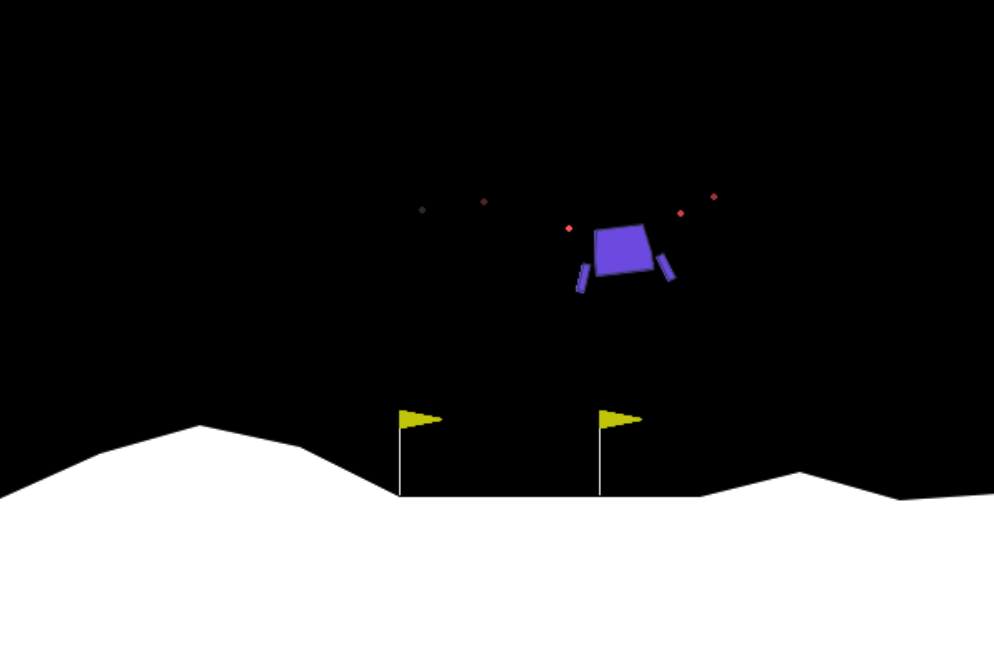
\includegraphics[width=0.45\linewidth]{figures/gym_landing.png}%
		\label{fig:landing}%
	}%
	\hfill%
	\subfloat[Ant MuJoCo environment]{%
		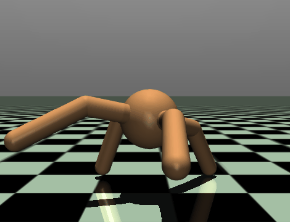
\includegraphics[width=0.45\linewidth]{figures/gym_ant_mujoco.png}%
		\label{fig:ant}%
	}%
	\caption{In figure \ref{fig:landing} (left) the goal is to land securely the spaceship (in pruple). In figure \ref{fig:translation_attn} (right) the goal is for the ant to balance itself and start walking.}
	\label{fig:faramas-gym}
\end{figure}

\subsection{Environment dynamics}
\label{sec:env_dyn}

The way that Farama's gym models agent-environment interaction is quite similar to what we explained in section \ref{sec:form-intro-rl}. In the listing \ref{code:init_env} we see a basic example of how an interaction with an environment can be performed. First, we need to instantiate the environment, calling the \inlinecode{gym.make} function, with the argument passed as the name of the environment we are going to interact. In order to initialize the environment, we must reset it, using the \inlinecode{env.reset()} method. Once we have our environment ready, we can proceed to interact with it performing actions. The number of actions, called action space, varies depending on the environment, but the gymnasium library offers methods and attributes that facilitate them in run-time, such as \inlinecode{env.action_space.n}. In the example provided, the action taken is random, using \inlinecode{env.action_space.sample()}, but we can use more complex methods to select the action our agent is going to perform (i.e. a neural network). 

\begin{lstlisting}[caption={Initialization of an environment in Farama's gymnasium}, label={code:init_env}]
import gymnasium as gym
env = gym.make("LunarLander-v2", render_mode="human")
observation, info = env.reset(seed=42)
for _ in range(1000):
	action = env.action_space.sample() 
	observation, reward, terminated, truncated, info = env.step(action)
	
	if terminated or truncated:
	observation, info = env.reset()

env.close()
\end{lstlisting}

In the RL framework, when an action is selected, the agent performs said action in the environment, and obtains a reward and a next observation. In the code, method \inlinecode{env.step()} is in charge of doing so, simulating what the outcome will be, returning the following:

\begin{itemize}
	\item \textbf{Observation}: What the environment lets the agent see about its state. If $\text{state}=\text{observation}$ then the environment is a MDP, if not, then its a POMDP.
	\item  \textbf{Reward}: The numerical signal that represents how good (or bad) the actions the agent is taking are.
	\item \textbf{Terminated}: Boolean flag that represents if the episode has ended.
	\item  \textbf{Truncated}: Boolean flag that represents if there has been an unexpected situation that resulted in the current episode ending prematurely. 
	\item \textbf{Info}: Additional information from the current state of the environment, such as current lives if the game is a survival, the current score or even and additional final observation if the state is terminal.
\end{itemize}

The interacting loop could go forever if no additional condition is stated, that is why using the truncated and terminated flags is the common approach to reset the environment and start a new episode. Once the simulation is over, we can close the environment using the \inlinecode{env.close()} method.

\subsection{Processing techniques of an environment}
\label{sec:proc_env}

In most of the environments, observations are usually RGB frames displaying the current situation of the environment. Since our models deal with visual data, it is quite convenient to use some pre-processing techniques that simplify the observation into something that is more "consumable" by the DQN agent. Farama's gymnasium provides an API that allows modifications of the environment, called \textbf{wrappers}. These wrappers are conceived so that they can alter the original behaviour of the environment, in terms of the reward, number of frames skipped between steps or the colour gamut of the observation. 

In our implementation, we make use of four custom wrappers, along with some pre-defined offered by the gymnasium library. This will ease the observation processing a make lightweight computations by discarding redundant information provided by the environment. In the following section we explain some of the custom wrappers that we have developed, along with some pre-defined ones.

\subsubsection{Skip N-Frames}
\label{sec:skip_wrapper}
In a RL environment, the variation between two consecutive frames usually is very little. If we pass each observation the environment provides, we end up with lots of redundant information which means that lots of computational resources are used in vane. One of the main approaches that is done in RL and other fields such as robotics or autonomous driving, where high frequency sensors are used is to skip a fixed amount of frames per observation. This technique is usually known as "frame skipping". The code developed for this wrapper is shown in listing \ref{code:skip_wrapper}. One thing to note is that in terms of reward, we add in the n-th frame the accumulated rewards from the skipped observations, since we are comprising the information of n-frames in just one observation.

\begin{lstlisting}[caption={Frame skip wrapper}, label={code:skip_wrapper}]
class SkipFrame(gym.Wrapper):
	def __init__(self, env: gym.Env, skip):
	"""Returns only the `skip`-th frame."""
		super().__init__(env)
		self._skip = skip
	
	def step(self, action):
	"""Repeat action, and sum reward"""
		total_reward = 0.0
		for _ in range(self._skip):
			obs, reward, done, trunk, info = self.env.step(action)
			total_reward += reward
			if done or trunk:
				break
	
	return obs, total_reward, done, trunk, info

\end{lstlisting}

\subsubsection{Gray-Scale Observation}
Most of the gymnasium's environments are in RGB colour coding. This may be useful for us humans, since we can extract additional information about the state of the game (i.e. detect if the ghosts in the Pac-man game are or colour blue or not, which gives us a hint on wether we can "eat" them and win points). Machine vision does not work like this, and this information sometimes is seen as redundant, since for a machine, the greyscale palette is enough. Also, it has its limitations in terms of computing power and resources. RGB images have three channels, which makes the observations more expensive to process, specially if we are stacking n-frames to them. Also, since we are dealing with experience replay models, storing these observations along with the collected experience can result in more memory consumption, which is not optimal in the training process. To solve this, the RGB observations are transformed to integer grey-scale. In this case, we are going to make use of PyTorch's transforms from the torchvision library that adds several visual transformations such as cropping, rotation, inversions or colour palette transformations. Using these transformations, we can also cast the original data-type of the observation (\inlinecode{numpy.array}) to a \inlinecode{torch.Tensor} datatype, which is convenient for processing said observation using a neural network using PyTorch framework. The code developed to apply this transformation to the environment is displayed in listing \ref{code:grayscale_wrapper}.

\begin{lstlisting}[caption={Grayscale frame wrapper}, label={code:grayscale_wrapper}]
class GrayScaleObservation(gym.ObservationWrapper):
	def __init__(self, env: gym.Env):
		super().__init__(env)
		obs_shape = self.observation_space.shape[:2]
		# since we are wrapping the observation that an environment provides,
		# we must update the observation space to match the new wrapped env.
		self.observation_space = Box(low=0, high=255, shape=obs_shape, dtype=np.uint8)
	
	def permute_orientation(self, observation):
		# permute [H, W, C] array to [C, H, W] tensor for pytorch model
		observation = np.transpose(observation, (2, 0, 1))
		observation = torch.tensor(observation.copy(), dtype=torch.float)
		return observation
	
	def observation(self, observation):
		observation = self.permute_orientation(observation)
		# since we have updated the observation space attribute, we must 
		# do so with the pixels from the env, casting them from RGB to grayscale
		transform = T.Grayscale()
		observation = transform(observation)
		return observation
	
\end{lstlisting}

\subsubsection{Resize Observation}
The size of an image is a crucial element in neural networks for visual data processing, a larger image is preferable, but it also comes at a cost, specially in the training stage. High resolution images require deeper and bigger models to capture all the spatial features, which results in more parameters to adjust during training. The issue comes with the availability of computational resources, since we do not have a cluster with multiple GPUs at our disposal. To adapt to our computational resources, we have added an additional custom wrapper to our environment that resizes the observation from its original shape, $256 \times 240$ to a down-scaled shape of $84 \times 84$. The code for doing so is portrayed in listing \ref{code:resize_wrapper}, where we use torchvision's transforms for doing so. Additionally, we normalize the pixel values by using the \inlinecode{T.Normalize(0,255)} transform.

\begin{lstlisting}[caption={Resize frame wrapper}, label={code:resize_wrapper}]
class ResizeObservation(gym.ObservationWrapper):
	def __init__(self, env: gym.Env, shape):
		super().__init__(env)
		# If shape is just a number it creates a tuple with that same number (i.e. 84 -> (84,84))
		# if is a list creates a "tuple" object with the given shape
		if isinstance(shape, int):
		self.shape = (shape, shape)
		else:
		self.shape = tuple(shape)
		
		obs_shape = self.shape # + self.observation_space.shape[:2]
		self.observation_space = Box(low=0, high=255, shape=obs_shape, dtype=np.uint8)
	
	def observation(self, observation):
		# Use torch transforms to resize the observation 
		# to the wanted resize resolution
		transforms = T.Compose(
			[T.Resize(self.shape, antialias=True),
			T.Normalize(0,255)]
		)
		
	# apply the transformation
	observation = transforms(observation).squeeze(0)
	return observation
	
\end{lstlisting}

\subsubsection{Additional Wrappers}
Additionally, there are some libraries such as Stable Baselines 3 \cite{stable-baselines3} or TorchRL \cite{bou2023torchrl} that provide methods and classes that encapsulate lots of the functionality provided by wrappers which were useful for our experiments:

\begin{itemize}
	\item \textbf{ClipRewardEnv}: Maps the original reward signal from the environment to the range [-1, 1]. This has multiple benefits, such as preventing larger gradients that may affect learning due to outliers in the reward distribution or encourage exploration, since the algorithm will not always go for high-reward actions, since all of them are within a small range. This is further explored in works such as \cite{Eschmann2021} where they remark the importance of designing an optimal reward signal for the agent to boost its behaviour.
	\item \textbf{EpisodicLifeEnv}: For games where the agent has several lives, treats losing a life as the end of the episode. This was originally implemented by Silver \textit{et al.} in \cite{mnih2013playing} to help the agent with value estimation.
	\item \textbf{MaxAndSkipEnv}: Frame skipping with some truncated behaviour (similar to what we have already explained in section \ref{sec:skip_wrapper}).
	\item \textbf{NoopResetEnv}: Once the environment is reset, during a certain amount of steps, the agent performs no actions (\textbf{no-op}erations) over the environment.
\end{itemize}

 While it may be true that RL is not the field in AI that receives the most attention, little by little, lots of frameworks and libraries that make quite easy train a model are being launched. Both TorchRL and Stable Baselines are quite useful libraries, and since they are PyTorch oriented, they helped us quite a lot in the development of this work.

\section{Agents development}
\label{sec:agents_dev}

\subsection{DQN  and DDQN training loop}
\label{sec:dqn_training_loop}
\subsubsection{Explaining the algorithm}
Once we had our environment ready for the agent to play, we proceeded to develop the DQN algorithm as Silver \textit{et al.} defined in \cite{mnih2013playing}. In this section we will first explain the algorithm and the we will briefly explain how we program it using pure python and PyTorch.

\begin{algorithm}
	\caption{DQN with Experience Replay}
	\label{alg:dqn}
	\begin{algorithmic}[1]
		\State Initialize replay memory $D$ to capacity $N$
		\State Initialize action-value function $Q$ with random weights
		\State Initialize target action-value function $\hat{Q}$ with weights $\theta^{-} = \theta$
		\For{episode = 1, $M$}
		\State Initialize sequence $s_1 = \{x_1\}$ and pre-processed sequence $\phi_1 = \phi(s_1)$
		\For{t = 1, $T$}
		\State With probability $\epsilon$ select a random action $a_t$
		\State otherwise select $a_t = \arg\max_a Q(\phi(s_t), a; \theta)$
		\State Execute action $a_t$ in emulator and observe reward $r_t$ and image $x_{t+1}$
		\State Set $s_{t+1} = s_t, a_t, x_{t+1}$ and preprocess $\phi_{t+1} = \phi(s_{t+1})$
		\State Store transition $(\phi_t, a_t, r_t, \phi_{t+1})$ in $D$
		\State Sample random mini-batch of transitions $(\phi_j, a_j, r_j, \phi_{j+1}) \sim D$
		\State Set $y_j = 
		\begin{cases} 
			r_j & \text{if episode terminates at step } j+1 \\
			r_j + \gamma \max_{a'} \hat{Q}(\phi_{j+1}, a'; \theta^{-}) & \text{otherwise}
		\end{cases}$
		\State Perform a gradient descent step on $(y_j - Q(\phi_j, a_j; \theta))^2$ with respect to the network parameters $\theta$
		\State Every $C$ steps reset $\hat{Q} = Q$
		\EndFor
		\EndFor
	\end{algorithmic}
	
\end{algorithm}

The algorithm is defined in \ref{alg:dqn}, where first we define a replay memory. This replay memory is basically a data structure that focus on storing experiences that the agent performs in the environment. Formally, we define as experience the tuple as $(\phi_t, a_t, r_t, \phi_{t+1})$, although when developing the code, we made some minor adjustments for better performance and extended functionality, such as store if the experience resulted in a terminal state. Also, we initialize our action-value function approximator $Q$ with random weights, which we will call the online approximator. From there, we will create our target network (the look-ahead), that will be defined as $\hat{Q}$ and copy the weights $\theta$ from $Q$ (the online/estimation network) to $\hat{Q}$. This ensures that the online function approximator and the target function approximator start the training process under equal circumstances, avoiding inaccurate estimation for the state-action values.

Once these initialization steps are done, we begin the training loop, where we iterate for a fixed number of episodes $N$ in the training process. Since we want to extract the most relevant features, we assume that there is a function $\phi$ that will pre-process the environment, extracting the most relevant features from our input $x_t$ creating the feature vector $s_t$. For us, this would be the wrappers explained in section \ref{sec:proc_env}. Then, the episode begin and, for each time step t, up until the episode ends (the agent finds itself in a terminal state) the agent starts playing and learning.

Both DQN and DDQN follow an $\epsilon$-greedy policy as the behavioural policy $\pi$, meaning that with a probability $\epsilon$ a random action will be selected instead of the one most rewarding one, according to our $Q$-value estimation. This encourage exploration, and not falling into a sub-optimal set of $Q$-values as explained in \cite{exploitation_vs_exploration}, where the exploration vs. exploitation dilemma is discussed. For our implementation, we will have and initial exploration rate $\epsilon_0$ and a final exploration rate $\epsilon_f$ and we designed a scheduling that decays the value of $\epsilon$. Doing so provides an exploration stage at first, where the agent is forced to perform lots of random actions, experimenting and evaluating different situations, thus, increasing the variability of the states that it can learn from.

Once the action is performed, the environment will react to it, providing a reward for such action and a new raw observation $x_{t+1}$. This will create a transition tuple that will be stored in the replay memory buffer $D$. 

As DQN is an off-policy algorithm, we will learn by performing actions that do not follow the behavioural policy $\pi$ but the target policy $\mu$. By doing so, we will sample a transition tuple from the replay memory $D$, and applying the greedy policy obtaining the $Q$-values obtained as the target $y_j$ for the $s_{t+1}$ (the look-ahead) of the sampled transition tuple. For the online network, we will compute the $Q$-values for the current state $s_t$ and apply action selection using the greedy policy, obtaining the agent estimations for the current state. As explained in section \ref{sec:val-fun_approx}, by minimizing this loss as the TD-error, we are teaching the online network to base the value estimations of the current state $s_t$ using the target network estimations $s_{t+1}$. This could be seen as a "look-ahead" view that glances into the "future" to obtain more information about how good the current state is. Once we got loss value, we adjust the online network weights $\theta$ to minimize the loss using the gradient descent algorithm. 

Finally, when a fixed number of steps has passed, we will copy the online network parameters $\theta$ onto the target network, so that the distribution of the parameters from the target network do not diverge too much from the online network.

\subsubsection{Main loop implementation}
While the DQN algorithm seems quite straight forward on paper, the implementation tells other story. For doing so, we implemented several modules to compartmentalize the different functionalities. By making the code modular, the process of improving the code, add new functionalities and connect different modules was easier, creating a pipeline that allowed to test several training set-ups in parallel.

The main script is called \href{https://github.com/Javimh18/DL_TFM/blob/main/src/train.py}{train.py} which basically loads all the hyper-parameters that the code needs, such as $\gamma$ for the target estimation or the learning rate when adjusting the net hyper-parameters given the loss. After that, it initializes the agent, that can be of two types, DQN or DDQN to then pass all these arguments into the \href{https://github.com/Javimh18/DL_TFM/blob/main/src/trainer.py}{Trainer} class. This class implements the main functionality explained in algorithm \ref{alg:dqn}, and a code snippet is presented in listing \ref{code:trainer_main_loop}. We will go deeper into this class in the following sections, but for now we will only explain the main functionality. First, we reset the environment, and using the done and truncated flags provided by the agent, we can check whether the episode finishes or not. Then, the agent performs an action according to the action-state values over the environment, obtaining a transition tuple which is stored in the replay memory. Finally, the agent learns from the pool of experiences stored in the replay buffer.

\begin{lstlisting}[caption={Trainer main loop}, label={code:trainer_main_loop}]
while self.curr_step < self.n_steps:
	# reset environment
	done, trunc = False, False
	state = self.env.reset()
	#measure_array = []
	while (not done) and (not trunc):
		# 1. get action for state
		action = self.agent.perform_action(state, self.curr_step)  
		# 2. run action in environment
		next_state, reward, done, trunc, info = self.env.step(action) 
		# 3. collect experience in exp. replay buffer for Q-learning
		self.agent.store_transition(state, action, reward, next_state, done, trunc) 
		# 4. Learn from collected experiences
		q, loss = self.agent.learn(self.curr_step)
		# 5. Update the current state 
		state = next_state
		# 6. Update step value 
		self.curr_step += 1            
		logger.log_step(loss, q)

	if 'episode' in info:
		# episode field is stored in the info dict if episode ended
		logger.log_episode(ep_length=info['episode']['l'], ep_reward=info['episode']['r'],)
		if not(self.curr_episode % self.log_every) :
			logger.record(episode=self.curr_episode, 
									epsilon=self.agent.exploration_rate, 
									step=self.curr_step)
			# log the real reward using episode statistics
		self.curr_episode += 1
	
\end{lstlisting}

\subsubsection{Digging deeper: the DQN agent}
\label{sec:digging_dqn_agent}

Once we have seen the training loop, we are going to delve into the agent functionality (\href{https://github.com/Javimh18/DL_TFM/blob/main/src/agents/dqn_agent.py}{dqn\_agent.py}). 

\begin{lstlisting}[caption={Perform action method from the DQN Agent}, label={code:ex_action}]
@torch.no_grad()
def perform_action(self, state, t):
	# decide wether to exploit or explore
	if np.random.random() < self.exploration_rate:
		action =  np.random.randint(0, self.action_dim)
	else:
		# use of __array__(): https://gymnasium.farama.org/main/_modules/gymnasium/wrappers/frame_stack/
		state = first_if_tuple(state).__array__()
		state = torch.tensor(state, device=self.device).unsqueeze(0)
		q_values = self.net(state, model='online')
		action = torch.argmax(q_values, dim=1).item()
	
	# decrease exploration_rate according to scheduler
	self.exploration_rate = self.exp_scheduler.step(t)
	self.exploration_rate = max(self.exploration_rate_min, self.exploration_rate)
	
	return action
\end{lstlisting}

As we have seen in the listing \ref{code:trainer_main_loop}, the first thing that our agent does is execute an action. According to algorithm \ref{alg:dqn}, we perform the action according to the target policy. We can see the code in the listing \ref{code:ex_action} the \inlinecode{perform\_action} method when we pick the action that maximizes the action values. After that, we update the exploration scheduler. The exploration scheduler updates the exploration rate $\epsilon$ for each time-step with the \inlinecode{step}. We have used three different types of functions to do so: exponential, linear and product of exponentials, which we will talk about in following sections. After the agent selects the action, we store the transition in the replay memory module of the agent using the \inlinecode{store\_transition}. In our case, we opted to use \inlinecode{TensorDictReplayBuffer} module from TorchRL, since it has seamless integration with PyTorch, making it quite easy to use and efficient to run, as we can store the replay memory in the GPU, avoiding for bottlenecks in the training process runtime. Inside, this implementation of the replay buffer stores an array of transition tuples as tensors. When the agent samples from the replay memory, it can be done using mini-batches, making the training process more efficient. In the listing \ref{code:replay_memory_dqn} we define the replay memory buffer, where we can state the size of the memory in terms of transition tuples, the device where the replay memory is stored, the sampler or if the replay memory has a mapping to disk in case we have limited storage resources. Additionally, we can also define the algorithm to follow in the sampling process. In our case, we opted to use prioritized experience replay sampling \cite{schaul2016prioritized} which basically prioritizes more significant experiences based on higher temporal-difference errors during training, enhancing learning. The motivation behind this work is similar to what happens in unbalanced datasets, as the less frequent classes usually are the hardest to recognize for the classifier. In order to mitigate this, different techniques ensure to weight more importance sampling to the less frequent instances in the dataset. 

\begin{lstlisting}[caption={Code snippet for the replay memory of the DQN agent}, label={code:replay_memory_dqn}]
# defining the memory (experience replay) of the agent
self.memory = TensorDictReplayBuffer(storage=LazyMemmapStorage(
	max_size=float(agent_config['replay_memory_size']),
	scratch_dir='./memmap_dir',
	device=self.device,
	),sampler=PrioritizedSampler(max_capacity=int(float(agent_config['replay_memory_size'])), 
	alpha=1.0, 
	beta=1.0)
)
\end{lstlisting}

Storing different experiences along the exploration stage tries to ensure that by the time the agent starts to learn by back-propagation, there is enough data variability to capture enough different situations in the environment to learn to act in most of them. In our implementation, the learning process is done by the \inlinecode{learn} method from the agent class. We present the function in listing \ref{code:learn_dqn_fun}, where first, we have a series of if statements that check several conditions. The first if statement checks that a fixed number of steps has passed in the training to synchronize the online and target network parameters (i.e. $\theta_{online} \rightarrow \theta_{target}$). After that, we check if a fixed number of training steps has passed to save the state of the network periodically. In order to fill the replay memory buffer before start to learn from it, we define a number of steps where the network does nothing, called burning, that ensures that, by the time the network starts to adjust its weights, there is enough variability of experiences to learn from. Also, for computational resources purposes, we made the network learn only every \inlinecode{learn_every} steps.

\begin{lstlisting}[caption={\inlinecode{learn} function from the DQN agent}, label={code:learn_dqn_fun}]
def learn(self, step):
	
	# Once the error is computed, each sync_every the weights of the 
	# target network are updated to the online network
	if not (step % self.sync_every):
		self.sync_Q_target()
	
	# save the model each save_every steps
	if not (step % self.save_every) and step > 0:
		self.save(step)
	
	# Burning lets episodes pass but collects experiences for the memory buffer
	if step < self.burning:
		return None, None
	
	# Not learning every step, but every "learn_every" steps
	if step % self.learn_every != 0:
		return None, None
	
	state, action, reward, next_state, done, _ = self.recall()
	
	# once we have our transition tuple, we apply TD learning over our DQN and compute the loss
	q_estimate = self.compute_q_estimate(state, action)
	q_target = self.compute_q_target(reward, done, next_state)
	
	# update the q_online network using the loss
	loss = self.loss_fn(q_target, q_estimate) # Compute Huber loss
	self.optimizer.zero_grad()
	loss.backward()
	self.optimizer.step()
	
	return q_estimate.mean().item(), loss.item()
\end{lstlisting} 

After these checks, we start with the learning process. To do so, we first recall or sample from the replay buffer with a defined sample size (i.e. 8, 16, 32... etc.) that extract a set of samples for the model to learn. Thanks to tensor operation support provided from PyTorch, this is forwarded through the online and target networks seamlessly. The \inlinecode{compute\_q\_target} method implements the TD target element in the DQN loss equation \ref{eq:dqn_loss} which is $r + \gamma \max_{a'} Q(s', a'; w^-))$, while the method \inlinecode{compute\_q\_estimate} implements the TD estimate which is $Q(s, a; w)$ where actions $a$ and $a'$ are selected according to the target greedy policy for the sampled state s from the buffer and its corresponding next state s'.

With the TD values, we compute the loss. We opted for the Huber Loss \cite{9918637}, defined in equation \ref{eq:hub_loss} where $\delta$ is a regularization parameter. This type of loss is useful in these set-ups, thanks to its robustness to outliers in the data compared to the mean squared error loss function, which is of convenience for this problem in cases where loss between Q values estimates fall far over the hyper-parameter $\delta$.

\begin{equation}
	\label{eq:hub_loss}
	L_{\delta}(y, f(x)) = 
	\begin{cases} 
		\frac{1}{2}(y-f(x))^2 & \text{for $|y-f(x)| \leq \delta$, } \\
		\delta \cdot \left(|y-f(x)| - \frac{1}{2}\delta \right) & \text{otherwise}
	\end{cases}
\end{equation}

Finally, once the loss is computed, we perform the back-propagation process in the online network to adjust its weights and we return the mean Q-values for the sampled mini-batch.

\subsubsection{DDQN training loop: A minor update}
\label{sec:ddqn_training_loop}
In \cite{vanhasselt2015deep}, Van Hasselt \text{et al.} proposed an updated version of the DQN algorithm. As explained in section \ref{sec:val-fun_approx}, the overestimation bias from the DQN comes from the target evaluating and selecting the actions from the target network. To mitigate this, they propose to decouple the action selection for the TD-target, using the online network and evaluating that action with the target network. We apply the same changes for the DDQN agent as can be seen in listings \ref{code:dqn_action_selection} and \ref{code:ddqn_action_selection}. Since the functionality of the DDQN agent is exactly the same as the DQN, except for the TD target value, we made the DDQN agent class inherit from the DQN agent in the \href{https://github.com/Javimh18/DL_TFM/blob/main/src/agents/ddqn_agent.py}{ddqn\_agent.py} script, taking advantage of the already developed code.

\begin{lstlisting}[caption={DQN action selection algorithm}, label={code:dqn_action_selection}]
@torch.no_grad() # since this is our "ground truth" (look ahead prediction)
def compute_q_target(self, reward, done, next_state):
	q_next_max_value, _ = torch.max(self.net(next_state, model='target'), dim=1)
	return reward + (1 - done.float()) * self.gamma * q_next_max_value
\end{lstlisting}

\begin{lstlisting}[caption={DDQN action selection algorithm}, label={code:ddqn_action_selection}]
@torch.no_grad() # since this is our "ground truth" (look ahead prediction)
def compute_q_target(self, reward, next_state, done):
	# for the next state, get the actions that have higher q_values
	online_q_action_value = self.net(next_state, model='online')
	max_value_action = torch.argmax(online_q_action_value, dim=1)
	# then, apply those actions onto the target (off-line) model
	target_q_action_values = self.net(next_state, model='target')
	q_next_max_value = target_q_action_values[np.arange(0, self.batch_size), max_value_action]
	
	return (reward + (1-done.float()) * self.gamma * q_next_max_value).float()
\end{lstlisting}

\subsection{Attention-based models: Vision Transformer}
\label{sec:vit_transformer_imp}
The aim of this work is to test out if there is any explain-ability in the decision making that agents perform when the value function is an approximator, which is an ideal set-up for DQN learning. For this section we will discuss the implementation of the attention-based models (i.e. vision transformers) that were used to carry out our experiments. First, we will talk about the Vision Transformer, discussing about the relevant aspects involved from the intuition to the actual implementation, that we took from \cite{caron2021emerging}. 

In several implementations for the vision transformer, we see that one of the most important things is for the model to be flexible to different configurations, where the number of blocks, embedding dimension or the number of heads in the multi-head attention block changes. This leads to easier ways to try out different configurations for the training process. For this section, first we are going to go over the constructor of the model and discuss its several parts. After that we will delve in the implementation of the most relevant.

\subsubsection{Constructor}
The constructor of the ViT is portrayed in listing \ref{code:vit_constructor}. We can see that the class is flexible to parametrizations, since we can specify the image size, the patch size, the channel of the input or the embedding dimension. In general terms, the constructor initializes the patch embedding module. This component is in charge of taking the input image and extract the patches from the spatial coordinates while enlarging the channel dimension from in channels to the embedding dimension. After that, it declares two essential parameters for the ViT: the class token and the positional embedding, which both of them are self learnable parameters that the network adjust during training. The next main component is a sequence of ViT blocks, which are implementations of the transformer encoder which are stacked one on top of each other. Finally, we have the classification head, which maps from the embedding dimension of the class token vector to the output dimension of the network, producing the corresponding Q value of an action as an output. We would also like to notice that for this implementation to work with the DDQN algorithm, we made some minor adaptations to the code, such as adding some additional dense layers to map from the feature space to the action space.

\begin{lstlisting} [caption={ViT model initialization}, label={code:vit_constructor}]
def __init__(self, img_size=224, patch_size=16, in_chans=3, num_classes=0, embed_dim=768, depth=12,
	num_heads=12, mlp_ratio=4., qkv_bias=False, qk_scale=None, drop_rate=0., attn_drop_rate=0.,
	drop_path_rate=0., norm_layer=nn.LayerNorm, **kwargs):
	super().__init__()
	self.num_features = self.embed_dim = embed_dim
	
	self.patch_embed = PatchEmbed(
	img_size=img_size, patch_size=patch_size, in_chans=in_chans, embed_dim=embed_dim)
	num_patches = self.patch_embed.num_patches
	
	self.cls_token = nn.Parameter(torch.zeros(1, 1, embed_dim))
	self.pos_embed = nn.Parameter(torch.zeros(1, num_patches + 1, embed_dim))
	self.pos_drop = nn.Dropout(p=drop_rate)
	
	dpr = [x.item() for x in torch.linspace(0, drop_path_rate, depth)]  # stochastic depth decay rule
	self.blocks = nn.ModuleList([
		Block(
		dim=embed_dim, num_heads=num_heads, mlp_ratio=mlp_ratio, qkv_bias=qkv_bias, qk_scale=qk_scale,
		drop=drop_rate, attn_drop=attn_drop_rate, drop_path=dpr[i], norm_layer=norm_layer)
		for i in range(depth)])
	self.norm = norm_layer(embed_dim)
	
	# Classifier head
	self.head = nn.Linear(embed_dim, num_classes) if num_classes > 0 else nn.Identity()
	
	trunc_normal_(self.pos_embed, std=.02)
	trunc_normal_(self.cls_token, std=.02)
	self.apply(self._init_weights)
\end{lstlisting}

\subsubsection{Patch Embedding}
The patch embedding module is of great importance, since it is what transforms the visual data into something that is "consumable" for the ViT. The code of the patch embedding is in listing \ref{code:patch_embedding}. To perform the patch projections, they use a trick leveraging the 2D convolutional operator, where they specify the filter size and the stride as the size of the patch. This ensures that the projections are non-overlapping and reduced in the spatial dimension. Additionally, since we want the channels to be projected from the \inlinecode{in\_channels} dimension to the embedding dimension, the number of filters specified in the 2D convolution operator is the same as the embedding dimension. With this trick, the implementation is more efficient and readable, providing the embedded patches from the original image.

\begin{lstlisting}[caption={Patch Embedding module}, label={code:patch_embedding}]
class PatchEmbed(nn.Module):
	""" 
	Image to Patch Embedding
	"""
	def __init__(self, img_size=224, patch_size=16, in_chans=3, embed_dim=768):
	super().__init__()
	num_patches = (img_size // patch_size) * (img_size // patch_size)
	self.img_size = img_size
	self.patch_size = patch_size
	self.num_patches = num_patches
	
	self.proj = nn.Conv2d(in_chans, embed_dim, kernel_size=patch_size, stride=patch_size)
	
	def forward(self, x):
		B, C, H, W = x.shape
		x = self.proj(x).flatten(2).transpose(1, 2)
		return x
\end{lstlisting}

\subsubsection{ViT encoder block}
Once we have our embedded image, we can proceed to process it using the ViT encoder blocks. The code of a single block is depicted in listing \ref{code:vit_block_implementation}. The input of a single block is either the embedded input image of the previous block output, to which the self attention layer will be applied, or the original image embedded. We will delve into the implementation of the attention layer after, but for now, the only thing we ought to know is that the attention layer returns the input embedding pondered by the importance of each patch. After that, it applies an projection to a layer with four times the embedding dimension to then apply a dropout layer. Since these models are very deep, in the forward pass we see that a residual connection \cite{he2015deep} is implemented, that eases the gradient flow in the back-propagation stage.

\begin{lstlisting}[caption={ViT blocks implementation}, label={code:vit_block_implementation}]
class Block(nn.Module):
	def __init__(self, dim, num_heads, mlp_ratio=4., qkv_bias=False, qk_scale=None, drop=0., attn_drop=0.,
		drop_path=0., act_layer=nn.GELU, norm_layer=nn.LayerNorm):
		super().__init__()
		self.norm1 = norm_layer(dim)
		self.attn = Attention(
		dim, num_heads=num_heads, qkv_bias=qkv_bias, qk_scale=qk_scale, attn_drop=attn_drop, proj_drop=drop)
		self.drop_path = DropPath(drop_path) if drop_path > 0. else nn.Identity()
		self.norm2 = norm_layer(dim)
		mlp_hidden_dim = int(dim * mlp_ratio)
		self.mlp = Mlp(in_features=dim, hidden_features=mlp_hidden_dim, act_layer=act_layer, drop=drop)
	
	def forward(self, x, return_attention=False):
		y, attn = self.attn(self.norm1(x))
		if return_attention:
			return attn
		x = x + self.drop_path(y)
		x = x + self.drop_path(self.mlp(self.norm2(x)))
	return x
\end{lstlisting}

\subsubsection{ViT Attention Module}
The attention blocks are the core functionality of this model. The code from the implementation is in listing \ref{code:attn_block}. In the constructor of the module, we can see that to compute the dimension of each head, it divides the embedding dimension by the number of heads we are going to apply. After that, it defines the weight matrices of the query, key and value from the self-attention module. To do so, it uses another trick to reduce the number of the layer's weights, by multiplying by three the embedding dimension, and then rearranging the tensor, so the highest order dimension is the one which contains the query, key and value values of the attention layer. After that it performs the self-attention operation, according to the equation \ref{eq:attn_eq}, obtaining the pondered embeddings. Finally, it performs some additional linear projections to obtain the final embedding. One thing that is of great use from this ViT block is that, it also returns the attentions maps from the attention blocks.

\begin{lstlisting}[caption={Attention module for the ViT model}, label={code:attn_block}]
class Attention(nn.Module):
	def __init__(self, dim, num_heads=8, qkv_bias=False, qk_scale=None, attn_drop=0., proj_drop=0.):
		super().__init__()
		self.num_heads = num_heads
		head_dim = dim // num_heads
		self.scale = qk_scale or head_dim ** -0.5
		
		self.qkv = nn.Linear(dim, dim * 3, bias=qkv_bias)
		self.attn_drop = nn.Dropout(attn_drop)
		self.proj = nn.Linear(dim, dim)
		self.proj_drop = nn.Dropout(proj_drop)
	
	def forward(self, x):
		B, N, C = x.shape
		qkv = self.qkv(x).reshape(B, N, 3, self.num_heads, C // self.num_heads).permute(2, 0, 3, 1, 4)
		q, k, v = qkv[0], qkv[1], qkv[2]
		
		attn = (q @ k.transpose(-2, -1)) * self.scale
		attn = attn.softmax(dim=-1)
		attn = self.attn_drop(attn)
		
		x = (attn @ v).transpose(1, 2).reshape(B, N, C)
		x = self.proj(x)
		x = self.proj_drop(x)
		return x, attn
\end{lstlisting}

\subsubsection{The forward method}
With these main modules from the ViT explained, we can now address the \inlinecode{forward} method from the ViT class, which is portrayed in listing \ref{code:vit_forward}. First, the \inlinecode{forward} method calls \inlinecode{prepare_tokens}, which is a function that encapsulates the patch embedding functionality plus the initialization of the positional encoding and the concatenation of the token class to the patch embedding tensor, as shown in figure \ref{fig:attn_maps}. After that, the positional embedding is added to the embedded tensor, giving additional context on how the patches are arranged, to then be passed to the ViT blocks. The ViT blocks are held into a \inlinecode{ModuleList} type of object from PyTorch's library. This enables creating lists where each element is a \inlinecode{nn.Module}, which can be tracked down by PyTorch's graph engine to perform forward and backward passes. The code iterates over the list of blocks, to then obtain a normalized embedding using a \inlinecode{NormLayer} module. Finally, to project from the embedding class to the action space, we perform a linear projection and obtain the class token indexing by \inlinecode{x[:, 0]}.

\begin{lstlisting}[caption={ViT forward method}, label={code:vit_forward}]
def prepare_tokens(self, x):
	B, nc, w, h = x.shape
	x = self.patch_embed(x)  # patch linear embedding
	
	# add the [CLS] token to the embed patch tokens
	cls_tokens = self.cls_token.expand(B, -1, -1)
	x = torch.cat((cls_tokens, x), dim=1)
	
	# add positional encoding to each token
	x = x + self.interpolate_pos_encoding(x, w, h)
	
	return self.pos_drop(x)
	
def forward(self, x):
	x = self.prepare_tokens(x)
	for blk in self.blocks:
		x = blk(x)
	x = self.norm(x)
	x = self.head(x)
	return x[:, 0]
\end{lstlisting}

If the reader wants to see the code in depth, this implementation is in the \href{https://github.com/Javimh18/DL_TFM/blob/main/src/models/vit.py}{vit.py} script, under the models folder from the repository.

\subsection{Attention-based models: SWIN Transformer}
\label{sec:swin_transformer_rl}
In this section we will do something similar to section \ref{sec:vit_transformer_imp}, where first we will talk about the intuition the changes with respect to the vision transformer, and then we will go over the implementation of those changes, using the code from \cite{liu2021swin}, since this model is actually more complex in the development aspect that the ViT. Another thing to note is that we will not go over the whole code used and implemented for these models, instead, we will give a comprehensive review of the implementation and delve only into the most critical aspects of them.

The SWIN transformer emerged as a version of the ViT that takes into account hierarchical features, resembling the convolutional neural networks approach to solve vision problems. It is composed from different stages, that hold different blocks. Additionally, the model introduces spatial dimension reduction, which is a big change in terms of how the model interact and manipulates the data. Additionally, it introduces the concepts of windows in order to reduce the computational overhead of the self-attention operation. In listing \ref{code:swin_transformer_constructor} we a reduced version of the original implementation. 

\subsubsection{Constructor}
One of the main changes that the SWIN Transformer introduces is the positional embedding, which is relative between patches, instead of absolute as the ViT. The main reason behind this is the fact that the patches are now within windows, and the attention is computed within those windows, so each patch should have some kind of notion on where the other patches inside its window are. Additionally, the declaration of the SWIN layers follows exactly the same logic as the ViT, but with a minimal difference. According to figure \ref{fig:swinarchitecture} from section \ref{sec:swin-transformer} we want for each SWIN stage to have different SWIN transformer layers, and, at the end, a patch merging transformation to reduce the spatial dimension. To do so, the BasicLayer module contains a flexible set-up where parameters such as number of heads, the depth for each layer or the window size may vary depending on the stage where is declared. The implementation is also flexible to a variable number of BasicLayer layers, since it uses the \inlinecode{ModuleList} object.

\begin{lstlisting} [caption={SWIN Transformer constructor}, label={code:swin_transformer_constructor}]
class SwinTransformer(nn.Module):
	
	def __init__(self, img_size=224, patch_size=4, in_chans=3, num_classes=1000, embed_dim=96, depths=[2, 2, 6, 2], num_heads=[3, 6, 12, 24], window_size=7, mlp_ratio=4., qkv_bias=True, qk_scale=None, drop_rate=0., attn_drop_rate=0., drop_path_rate=0.1,	norm_layer=nn.LayerNorm, ape=False, patch_norm=True, use_checkpoint=False, **kwargs):
		super().__init__()
		
		# ... Already explained variables in VIT transformer + Patch Embedding
		
		# absolute position embedding
		if self.ape:
			self.absolute_pos_embed = nn.Parameter(torch.zeros(1, num_patches, embed_dim))
			trunc_normal_(self.absolute_pos_embed, std=.02)
		
		# ... Already explained variables in VIT transformer
		
		# build layers
		self.layers = nn.ModuleList()
		for i_layer in range(self.num_layers):
			layer = BasicLayer(dim=int(embed_dim * 2 ** i_layer),
						input_resolution=(patches_resolution[0] // (2 ** i_layer),
						patches_resolution[1] // (2 ** i_layer)),
						depth=depths[i_layer],
						num_heads=num_heads[i_layer],
						window_size=window_size,
						mlp_ratio=self.mlp_ratio,
						qkv_bias=qkv_bias, qk_scale=qk_scale,
						drop=drop_rate, attn_drop=attn_drop_rate,
						drop_path=dpr[sum(depths[:i_layer]):sum(depths[:i_layer + 1])],
						norm_layer=norm_layer,
						downsample=PatchMerging if (i_layer < self.num_layers - 1) else None,
						use_checkpoint=use_checkpoint)
			self.layers.append(layer)
			
		# ... Already explained variables in VIT transformer
		
		self.apply(self._init_weights)
\end{lstlisting}

\subsubsection{BasicLayer}
The \inlinecode{BasicLayer} module has inside of it the functionality that goes inside of every stage of the SWIN transformer. To do so, the class attribute \inlinecode{self.blocks} is declared as a \inlinecode{ModuleList} where the \inlinecode{SwinTransformerBlock} instances are declared. Since at the end of some stages, the patch merging module is applied, the \inlinecode{down-sample} boolean flag indicates whether that stage performs down-sampling via patch merging or not. The forward method is pretty straight-forward, as the code first iterates through the  \inlinecode{SwinTransformerBlock} instances and then down-samples the spatial resolution of the returned embeddings if needed.

\begin{lstlisting}
class BasicLayer(nn.Module):

	def __init__(self, dim, input_resolution, depth, num_heads, window_size,
		mlp_ratio=4., qkv_bias=True, qk_scale=None, drop=0., attn_drop=0.,
		drop_path=0., norm_layer=nn.LayerNorm, downsample=None, use_checkpoint=False):
		
		super().__init__()
		self.dim = dim
		self.input_resolution = input_resolution
		self.depth = depth
		self.use_checkpoint = use_checkpoint
		
		# build blocks
		self.blocks = nn.ModuleList([
			SwinTransformerBlock(dim=dim, input_resolution=input_resolution,
				num_heads=num_heads, window_size=window_size,
				shift_size=0 if (i % 2 == 0) else window_size // 2,
				mlp_ratio=mlp_ratio,
				qkv_bias=qkv_bias, qk_scale=qk_scale,
				drop=drop, attn_drop=attn_drop,
				drop_path=drop_path[i] if isinstance(drop_path, list) else drop_path,
				norm_layer=norm_layer)
		for i in range(depth)])
		
		# patch merging layer
		if downsample is not None:
			self.downsample = downsample(input_resolution, dim=dim, norm_layer=norm_layer)
		else:
			self.downsample = None
	
	def forward(self, x):
		for blk in self.blocks:
			if self.use_checkpoint:
			x = checkpoint.checkpoint(blk, x)
		else:
			x = blk(x)
		if self.downsample is not None:
			x = self.downsample(x)
		return x
\end{lstlisting}

\subsubsection{SwinTransformerBlock}
In the \inlinecode{SWINTransformerBlock} we have the core functionality of the SWIN transformer. The first part of the constructor is defined in listing \ref{code:swin_cons_part1}. We can see that the main part is the \inlinecode{WindowAttention} class, which we will explain in the following section.

\begin{lstlisting}[caption={First part of the SWIN block constructor}, label={code:swin_cons_part1}]
def __init__(self, dim, input_resolution, num_heads, window_size=7, shift_size=0,
	mlp_ratio=4., qkv_bias=True, qk_scale=None, drop=0., attn_drop=0., drop_path=0.,
	act_layer=nn.GELU, norm_layer=nn.LayerNorm):
	super().__init__()
	self.dim = dim
	self.input_resolution = input_resolution
	self.num_heads = num_heads
	self.window_size = window_size
	self.shift_size = shift_size
	self.mlp_ratio = mlp_ratio
	if min(self.input_resolution) <= self.window_size:
	# if window size is larger than input resolution, we don't partition windows
	self.shift_size = 0
	self.window_size = min(self.input_resolution)
	assert 0 <= self.shift_size < self.window_size, "shift_size must in 0-window_size"
	
	self.norm1 = norm_layer(dim)
	self.attn = WindowAttention(
	dim, window_size=to_2tuple(self.window_size), num_heads=num_heads,
	qkv_bias=qkv_bias, qk_scale=qk_scale, attn_drop=attn_drop, proj_drop=drop)
\end{lstlisting}

After that, in the second part of the constructor, displayed in listing \ref{code:swin_cons_part2}, handles the initialization of the window shifting for the \inlinecode{WindowAttention} model, which will be of crucial importance in order to properly arrange the context of the shifted parts of the image. To do so, it creates masks, which activate several parts of the image depending on the context, following the same scheme as explained in section \ref{sec:swin-transformer}. After that, it applies the window partitioning using the created mask. The window partition basically uses a projection of the patches that fall into the window size, which will be of use when computing the window attention.

\begin{lstlisting}[caption={Second part of the SWIN block model}, label={code:swin_cons_part2}]
	self.drop_path = DropPath(drop_path) if drop_path > 0. else nn.Identity()
	self.norm2 = norm_layer(dim)
	mlp_hidden_dim = int(dim * mlp_ratio)
	self.mlp = Mlp(in_features=dim, hidden_features=mlp_hidden_dim, act_layer=act_layer, drop=drop)
	
	if self.shift_size > 0:
		# calculate attention mask for SW-MSA
		H, W = self.input_resolution
		img_mask = torch.zeros((1, H, W, 1))  # 1 H W 1
		h_slices = (slice(0, -self.window_size),
		slice(-self.window_size, -self.shift_size),
		slice(-self.shift_size, None))
		w_slices = (slice(0, -self.window_size),
		slice(-self.window_size, -self.shift_size),
		slice(-self.shift_size, None))
		cnt = 0
		for h in h_slices:
			for w in w_slices:
				img_mask[:, h, w, :] = cnt
				cnt += 1
	
	mask_windows = window_partition(img_mask, self.window_size)  # nW, window_size, window_size, 1
	mask_windows = mask_windows.view(-1, self.window_size * self.window_size)
	attn_mask = mask_windows.unsqueeze(1) - mask_windows.unsqueeze(2)
	attn_mask = attn_mask.masked_fill(attn_mask != 0, float(-100.0)).masked_fill(attn_mask == 0, float(0.0))
\end{lstlisting}

Once the main components of the class are initialized, the \inlinecode{forward} (listing \ref{code:swin_block_fwd}) reshapes the input tensor from dimensions B, L, C, where B is the batch dimension, L is the length dimension that refers to the flattened number of patches from the input (usually as a product of the spatial dimensions: height and width) and C is the channels dimension. It reshapes the input into from the flattened form to its spatial counter-part in line 7, to apply the window shifting using the \inlinecode{torch.roll} operator. Once the image is shifted, the \inlinecode{window_partition} method projects a window that holds inside a specified number of patches. For each of those windows, the attention module computes the self-attention between the patches that fall into their corresponding windows. With the attention weights applied for each window, the \inlinecode{window_reverse} method merges the window projections, returning the granularity of the input to patches. Finally, the \inlinecode{torch.roll} operator does the shifting but in the reversed order, returning the input to its original form, but with each patch pondered by the attention weights computed for its corresponding window.

\begin{lstlisting}[caption={Forward method for the SWIN Block module}, label={code:swin_block_fwd}]
def forward(self, x):
	H, W = self.input_resolution
	B, L, C = x.shape
	assert L == H * W, "input feature has wrong size"
	
	shortcut = x
	x = self.norm1(x)
	x = x.view(B, H, W, C)
	
	# cyclic shift
	if self.shift_size > 0:
		shifted_x = torch.roll(x, shifts=(-self.shift_size, -self.shift_size), dims=(1, 2))
	else:
		shifted_x = x
		
	# partition windows
	x_windows = window_partition(shifted_x, self.window_size)  # nW*B, window_size, window_size, C
	x_windows = x_windows.view(-1, self.window_size * self.window_size, C)  # nW*B, window_size*window_size, C
	
	# W-MSA/SW-MSA
	attn_windows = self.attn(x_windows, mask=self.attn_mask)  # nW*B, window_size*window_size, C
	
	# merge windows
	attn_windows = attn_windows.view(-1, self.window_size, self.window_size, C)
	shifted_x = window_reverse(attn_windows, self.window_size, H, W)  # B H' W' C
	
	# reverse cyclic shift
	if self.shift_size > 0:
		x = torch.roll(shifted_x, shifts=(self.shift_size, self.shift_size), dims=(1, 2))
	else:
		x = shifted_x
		x = x.view(B, H * W, C)
	
	# FFN
	x = shortcut + self.drop_path(x)
	x = x + self.drop_path(self.mlp(self.norm2(x)))
	
	return x
\end{lstlisting}

\subsubsection{Window Attention}
\label{sec:window_attention}
The Window Attention module from the SWIN Transformer is probably what resembles the most from the ViT. The  two main differences in the SWIN transformer attention are the relative positional embedding, which was first proposed for this architecture, and the masked attention which preserves the spatial context in shited scenarios. The code is displayed in \ref{code:win_attention_constructor}. From lines 11 to 25 the relative positional index is initialized. The process to obtain it is quite convoluted, but the main intuition relies on understanding that, for each window, it is important for the patches to not only know where they are in the picture, but also know where the rest of them are. By giving the relative position, the model provides a richer framework to understand not only the position a single patch, but its position with respect to the rest of the patches inside the projected window. After this part, the model uses the masks to understand which part of the window patches does it need to compute the attention. The rest of the module is pretty similar to the standard self-attention code explained in the ViT.

\begin{lstlisting}[caption={Window attention module constructor}, label={code:win_attention_constructor}]
def __init__(self, dim, window_size, num_heads, qkv_bias=True, qk_scale=None, attn_drop=0., proj_drop=0.):
	
	super().__init__()
	self.dim = dim
	self.window_size = window_size  # Wh, Ww
	self.num_heads = num_heads
	head_dim = dim // num_heads
	self.scale = qk_scale or head_dim ** -0.5
	
	# define a parameter table of relative position bias
	self.relative_position_bias_table = nn.Parameter(
	torch.zeros((2 * window_size[0] - 1) * (2 * window_size[1] - 1), num_heads))  # 2*Wh-1 * 2*Ww-1, nH
	
	# get pair-wise relative position index for each token inside the window
	coords_h = torch.arange(self.window_size[0])
	coords_w = torch.arange(self.window_size[1])
	coords = torch.stack(torch.meshgrid([coords_h, coords_w]))  # 2, Wh, Ww
	coords_flatten = torch.flatten(coords, 1)  # 2, Wh*Ww
	relative_coords = coords_flatten[:, :, None] - coords_flatten[:, None, :]  # 2, Wh*Ww, Wh*Ww
	relative_coords = relative_coords.permute(1, 2, 0).contiguous()  # Wh*Ww, Wh*Ww, 2
	relative_coords[:, :, 0] += self.window_size[0] - 1  # shift to start from 0
	relative_coords[:, :, 1] += self.window_size[1] - 1
	relative_coords[:, :, 0] *= 2 * self.window_size[1] - 1
	relative_position_index = relative_coords.sum(-1)  # Wh*Ww, Wh*Ww
	self.register_buffer("relative_position_index", relative_position_index)
	
	self.qkv = nn.Linear(dim, dim * 3, bias=qkv_bias)
	self.attn_drop = nn.Dropout(attn_drop)
	self.proj = nn.Linear(dim, dim)
	self.proj_drop = nn.Dropout(proj_drop)
	
	trunc_normal_(self.relative_position_bias_table, std=.02)
	self.softmax = nn.Softmax(dim=-1)
\end{lstlisting}

\subsubsection{The forward method}

With all the main modules explained, we use the \inlinecode{forward} method as an overview of the model. The code is in listing \ref{code:forward_swin}. The \inlinecode{forward_features} method handles the feature extraction from the input image to the compressed attention-weight representation that the SWIN transformer blocks output. This features go then to the output head, that maps the embedding dimension to the output dimension, in our case the actions available in the environment.

\begin{lstlisting}[caption={Forward method for the SWIN Transformer}, label={code:forward_swin}]
def forward_features(self, x):
	x = self.patch_embed(x)
	if self.ape:
		x = x + self.absolute_pos_embed
		x = self.pos_drop(x)
	
	for layer in self.layers:
		x = layer(x)
	
	x = self.norm(x)  # B L C
	x = self.avgpool(x.transpose(1, 2))  # B C 1
	x = torch.flatten(x, 1)
	return x
	
def forward(self, x, head=None):

	x = self.forward_features(x)
	x = self.head(x)
	return x
\end{lstlisting}

As we can see, the SWIN transformer is a step-up in comparison to the ViT, with more complex and efficient ways to compute and extract relevant features using attention and spatial reduction. If the reader wants to see the code in depth, this implementation is in the \href{https://github.com/Javimh18/DL_TFM/blob/main/src/models/swin_transformer.py}{swin\_transformer.py} script, under the models folder from the repository.

\section{Setting up the pipeline}
\label{sec:set_pipeline}

Up until this point, all we have explained in this section is the algorithmic part on how we programmed the agent in order to learn, but that is not the only important thing when developing machine learning algorithms. Our implementation comprises several modules to provide the training framework additional information on how the training process is going, which models work best, and save the weights of the neural networks that help the agent to perform better in the environment. We have already explained in sections \ref{sec:dqn_training_loop}, \ref{sec:vit_transformer_imp} and \ref{sec:swin_transformer_rl}, which are the main parts which work together to train the different agent configurations that we propose. In this section we will delve into the critical aspects from that have taken part to develop them. 

\subsection{Trainer}
The trainer class is kind of the orchestrator of this work. Its main functionality is to coordinate the environment with the agent learning procedure while extracting relevant metrics and evidences of the agent's behaviour. Our environment has different wrappers added to them, that alter the behaviour and the dynamics of the environment, which may be an issue if the code is not properly adapted. In section \ref{sec:env_dyn} we explain the different types of wrappers that we used, but we have not explained the implications that they have in the way the agent behaves and the metric extraction. For example, our environment uses the \inlinecode{EpisodicLifeEnvironment} which basically treats each life of a game as an episode from the agent to learn, which helps the agent to improve its estimates of the rewards. The issue here is that when we extract the real statistics of the episode they come altered. To solve these problems we make use of the wrapper \inlinecode{RecordEpisodeStatistics} which collects the actual real statistics from the environment. This wrapper adds to additional information to the environment when the episode has ended. In listing \ref{code:trainer_info_episode}, that is taken from listing \ref{code:trainer_main_loop}, we can see that in the info dictionary, that is return for each \inlinecode{env.step(action)} call, there is a key called episode that opens up an embedded dictionary with information that is specific from the episode, such as the accumulated reward or the length of the episode which we extracted and saved for logging purposes. Additional information can be extracted too, such as the last frame that the agent saw.

\begin{lstlisting}[caption={Episodic information retrival from \inlinecode{RecordEpisodeStatistics} wrapper}, label={code:trainer_info_episode}]
if 'episode' in info:
	# episode field is stored in the info dict if episode ended
	logger.log_episode(ep_length=info['episode']['l'], ep_reward=info['episode']['r'],)
	if not(self.curr_episode % self.log_every) :
		logger.record(episode=self.curr_episode, 
		epsilon=self.agent.exploration_rate, 
		step=self.curr_step)
		# log the real reward using episode statistics
		self.curr_episode += 1
\end{lstlisting}

\subsection{Logger}
To record how well an agent is performing, a main performance indicator needs to be tracked: the reward. The issue is that, sometimes, we may encounter environments where the reward gets progressively sparser, occluding information about how well the agent understands the scene and the actions it may perform. For example, in the Pacman game, rewards are very common at the beginning, but as the game goes on, they become increasingly difficult to obtain and if we do not take this into account, it may seem like the agent is not learning, which may not be true. That is why, additional indicators such as the episode length, the loss or the mean Q values can be of use to have a better understanding on whether the agent is learning or not. To comprise all this information, we have developed the logger module (\href{https://github.com/Javimh18/DL_TFM/blob/main/src/utils/logger.py}{logger.py}). We must say that for this module, we took inspiration from \cite{feng2022mario}.

The constructor of the logger class (MetricLogger), is defined in listing \ref{code:metric_logger_class}, where define the main attributes that hold the relevant information that we want to monitor. First, we indicate to the logger if the agent to log is pre-trained and we are continuing the training or performing a fine-tuning or it is a fresh new training thanks to the \inlinecode{load_pre} flag. If so, we assume that in the \inlinecode{save_dir} path there is already information about a previous logged training, if not the a new log file is created under the indicated directory. Additionally, we define the episodic arrays, that hold the information for each episode and the smoothed episodic arrays, that take the moving average of the metrics extracted from the last 100 episodes. After that, we call the \inlinecode{self.init_episode} to indicate the logger that we are going to start logging a new episode.

\begin{lstlisting}[caption={MetricLogger class initialization}, label={code:metric_logger_class}]
class MetricLogger:
	def __init__(self, save_dir:Path, agent_type:str, load_pre=False):
	
	# paths for saving logs and plots
	self.save_log = save_dir / "log"
	if not load_pre:
		# create if not exists
		save_dir.mkdir(parents=True)
		with open(self.save_log, "w") as f:
			f.write(
				f"{'Episode':>8}{'Step':>11}{'Epsilon':>10}{'MeanReward':>15}"
				f"{'MeanLength':>15}{'MeanLoss':>15}{'MeanQValue':>15}"
				f"{'TimeDelta':>15}{'Time':>20}\n"
			)
	else:
		self.load_from_log(save_dir)
		self.save_dir = save_dir
		self.agent_type = agent_type
		
	# History metrics
	self.ep_rewards = []
	self.ep_lengths = []
	self.ep_avg_losses = []
	self.ep_avg_qs = []
	
	# Moving averages, added for every call to record()
	self.moving_avg_ep_rewards = []
	self.moving_avg_ep_lengths = []
	self.moving_avg_ep_avg_losses = []
	self.moving_avg_ep_avg_qs = []
	self.steps = []
	
	# Current episode metric
	self.init_episode()
	
	# Timing
	self.record_time = time.time()
	
	def init_episode(self):
		self.curr_ep_loss = 0.0
		self.curr_ep_q = 0.0
		self.curr_ep_loss_length = 0
\end{lstlisting}

As our agent starts to perform actions, metrics will start to pop up. In order to monitor in the step and in the episode domain, we have two functions \inlinecode{log_step} and \inlinecode{log_episode}, defined in listing \ref{code:log_step_ep}, that compute the step information and record it in the episodic arrays defined in the constructor of the class. This information is stored from the beginning of the training up until the very end, but is not yet dumped into the log file. Once thing to notice is that, for the \inlinecode{log_step} function, we only accumulate the values if a loss is provided. If we recall the training procedure, the agent does not learn every step, but every fixed number of steps which helps with the computational over-head. When the agent is not learning, the loss is return as a \inlinecode{NoneType} object, hence, not recording the step metrics in the logger.

\begin{lstlisting}[caption={Step and episode functions for metrics extraction}, label={code:log_step_ep}]
def log_step(self, loss, q):
	"Mark end of step if loss is provided"
	if loss:
		self.curr_ep_loss += loss
		self.curr_ep_q += q
		self.curr_ep_loss_length += 1
	
def log_episode(self, ep_reward, ep_length):
	"Mark end of episode"
	self.ep_rewards.append(ep_reward)
	self.ep_lengths.append(ep_length)
	
	if self.curr_ep_loss_length == 0:
		ep_avg_loss = 0
		ep_avg_q = 0
	else:
		ep_avg_loss = np.round(self.curr_ep_loss / self.curr_ep_loss_length, 5)
		ep_avg_q = np.round(self.curr_ep_q / self.curr_ep_loss_length, 5)
		self.ep_avg_losses.append(ep_avg_loss)
		self.ep_avg_qs.append(ep_avg_q)
	
	self.init_episode()
\end{lstlisting}

To dump the information into the log file, we defined the \inlinecode{record} function, showed in listing \ref{code:log_record}. First, for all metrics, we compute the moving average of a window of 100 episodic values. This is because usually, training procedures in reinforcement learning (specially in TD learning) holds lots of variability, which sometimes result in noisy results. After that, we print via command line the statistics, for hands-on visualization. At last, we open the log file, and write the computed metrics, to then read it using a \inlinecode{pandas} data-frame, and plot the values using the \inlinecode{plotly} library, which has great integration with pandas data-frames for data plotting.

\begin{lstlisting}[caption={Record function, that saves the moving average statistics in the log file and plots the values of the statistics over the time-steps of the learning}, label={code:log_record}]
def record(self, episode, epsilon, step):
	mean_ep_reward = np.round(np.mean(self.ep_rewards[-100:]), 3)
	mean_ep_length = np.round(np.mean(self.ep_lengths[-100:]), 3)
	mean_ep_loss = np.round(np.mean(self.ep_avg_losses[-100:]), 3)
	mean_ep_q = np.round(np.mean(self.ep_avg_qs[-100:]), 3)
	self.moving_avg_ep_rewards.append(mean_ep_reward)
	self.moving_avg_ep_lengths.append(mean_ep_length)
	self.moving_avg_ep_avg_losses.append(mean_ep_loss)
	self.moving_avg_ep_avg_qs.append(mean_ep_q)
	self.steps.append(step)
	
	last_record_time = self.record_time
	self.record_time = time.time()
	time_since_last_record = np.round(self.record_time - last_record_time, 3)
	
	with open(self.save_log, "a") as f:
		f.write(
		f"{episode:8d}{step:10d}{epsilon:10.3f}"
		f"{mean_ep_reward:15.3f}{mean_ep_length:15.3f}{mean_ep_loss:15.3f}{mean_ep_q:15.3f}"
		f"{time_since_last_record:15.3f}"
		f"{datetime.datetime.now().strftime('%Y-%m-%dT%H:%M:%S'):>20}\n"
		)
	df = pd.read_csv(self.save_log, header=0, sep='\s+', skipinitialspace=True)
	for i in df.columns:
		if i not in NOT_2_PLOT:
			fig = px.line(df, x = 'Step', y = i, title=f'{i} over time for {self.agent_type}')
			fig.write_image(self.save_dir / f"{i}.png")
\end{lstlisting} 

The logger is one of the most useful tools that we have developed, since it can manage to monitor the training procedure seamlessly, even when several agents are being trained in parallel and allow us t better visualize the development of the agent's learning. 

\subsection{Schedulers}
In section \ref{sec:digging_dqn_agent}, we talked about how we have proposed three different exploration schemes for the $\epsilon$ value: linear decay, exponential decay and product of exponential decay. To formalize this, we proposed the equations \ref{eq:linear_sch}, \ref{eq:exp_sch} and \ref{eq:prod_exp_sch} for each type of schedule, $\epsilon_t$ is the current exploration rate for a time-step $t$,  $\epsilon_0$ is the initial exploration rate, $\epsilon_f$ is the final exploration rate, $N$ is the number of steps of exploration, $\lambda$ is an hyper-parameter and $\gamma$ is an parameter that we need to infer, given the upper bound $\epsilon_0$ and the lower bound $\epsilon_f$. 

\begin{equation}
	\label{eq:linear_sch}
	\epsilon_t = \frac{\epsilon_f - \epsilon_0}{N} \times t + \epsilon_0
\end{equation}

\begin{equation}
	\label{eq:exp_sch}
	\epsilon_t = \epsilon_0 \gamma_{exp}^{\lambda t}
\end{equation}

\begin{equation}
	\label{eq:prod_exp_sch}
	\epsilon_t = \epsilon_0 \prod_{i=0}^{t} \gamma_{prod}^{\lambda t}
\end{equation}

The $\gamma_{exp}$ value for the exponent decay function is defined in \ref{eq:gamma_exp}, where $\lambda$ is an hyperparameter, and the rest of the terms involved are the same as in equation \ref{eq:exp_sch}. On the other hand, the $\gamma_{prod}$ value for the product of exponents function is defined in  \ref{eq:gamma_pexp}, where $\lambda$ is an hyperparameter and $k$ is defined in equation \ref{eq:k_sum} as the general sum of the $N$ first values, where $n$ is the final value, $a_1$ is the first value and $d$ is the interval between the numbers of the sum, in this case 1.

\begin{equation}
	\label{eq:gamma_exp}
	\gamma_{exp} = \sqrt[\lambda N]{\frac{\epsilon_f}{\epsilon_0}}
\end{equation}

\begin{align}
	\gamma_{prod} = \sqrt[\lambda k]{\frac{\epsilon_f}{\epsilon_0}} \quad \label{eq:gamma_pexp}
\end{align}

\begin{equation}
	\label{eq:k_sum}
	k = \sum_{i=0}^{N} i  = n a_1 + d \frac{(n-1)n}{2}
\end{equation}

To clarify that the $\gamma$ used in these equations is completely different from the hyper-parameter that is used in the DQN learning equations defined in \ref{eq:dqn_loss} and \ref{eq:ddqn_loss}. Additionally, the way we came up with them is shown in section \ref{app:gamma_proof}.

To properly scheme the different schedulers, we first defined an abstract class, as seen in listing \ref{code:abs_scheduler}. This class has three main values, the upper bound \inlinecode{e_0}, the lower bound \inlinecode{e_f} and the number of time-steps for the function to go from the upper bound to the lower one. The step method will return the current exploration rate, given the current time-step.
\begin{lstlisting}[caption={Abstract class for the scheduler}, label={code:abs_scheduler}]
class Scheduler(ABC):
	def __init__(self, e_0, e_f, n_steps) -> None:
		self.e_0 = e_0
		self.e_f = e_f
		self.n_steps = n_steps
	@abstractmethod
	def step(self, t):
		pass
\end{lstlisting}

The implementation of the linear schedule in listing \ref{code:lin_scheduler} is pretty straight-forward. For each step, we pass the number of the time-step value, which would be the $t$ value for \ref{eq:linear_sch} and \ref{eq:exp_sch} equations and once we have computed the slope, we use as the y-intercept the upper bound \inlinecode{e_0}. 

\begin{lstlisting}[caption={Linear scheduler class}, label={code:lin_scheduler}]
class LinearScheduler(Scheduler):
	def __init__(self, e_0, e_f, n_steps) -> None:
		super().__init__(e_0, e_f, n_steps)
		self.slope = (e_f - e_0)/n_steps
	
	def step(self, t):
		e_t = self.slope*t + self.e_0
		return max(e_t, self.e_f)
\end{lstlisting}

The exponential decay schedule, displayed in listing \ref{code:exp_decay_scheduler}, is quite similar to the linear schedule. Instead of computing the slope, we compute the \inlinecode{gamma} value according to equation \ref{eq:gamma_exp}, but the rest is practically the same.

\begin{lstlisting}[caption={Exponential scheduler class}, label={code:exp_decay_scheduler}]
class ExpDecayScheduler(Scheduler):
	def __init__(self, e_0, e_f, n_steps) -> None:
		super().__init__(e_0, e_f, n_steps)
		self.gamma = (e_f / e_0)**(1/n_steps)
	
	def step(self, t):
		e_t = self.e_0 * self.gamma**t
		return max(e_t, self.e_f)
\end{lstlisting}

Finally, for the product of exponential decay schedule, displayed in listing \ref{code:prod_exp_decay_scheduler}, we had to compute the exploration rate in an efficient way to overcome efficiency problems. To do so, instead of looping through the multiplicative product, which would be computationally expensive, we defined an accumulator that held the values for each iteration, so that, when a new time-step comes in, we only have to multiply the accumulator by the exponent of the gamma to the time-step.

\begin{lstlisting}[caption={Product of exponentials decay schedule}, label={code:prod_exp_decay_scheduler}]
def gauss_sum(a:int, n:int, inc:float):
	return n/2*(2*a+(n-1)*inc)
	
class ProdExpDecayScheduler(Scheduler):
	def __init__(self, e_0, e_f, n_steps) -> None:
		super().__init__(e_0, e_f, n_steps)
	
		k = gauss_sum(a=0, n=n_steps, inc=1.0)
		self.gamma = (e_f / e_0)**(1/k)
		self.acc = e_0
	
	def step(self, t):
		self.acc *= self.gamma**t
		return max(self.acc, self.e_f)
\end{lstlisting}

To have a better understanding on how these equations behave over time, the shape of them is depicted in Figure \ref{fig:shape_exp_funs}, where $\gamma$ is the value computed according to the bounds of our exploration schedule. We came up with these different schedules to explore if they affect the exploration process when the agent is learning over the first steps. We will discuss more about this in Section \ref{cha:evaluation}.

\begin{figure}[!h]
	\centering
	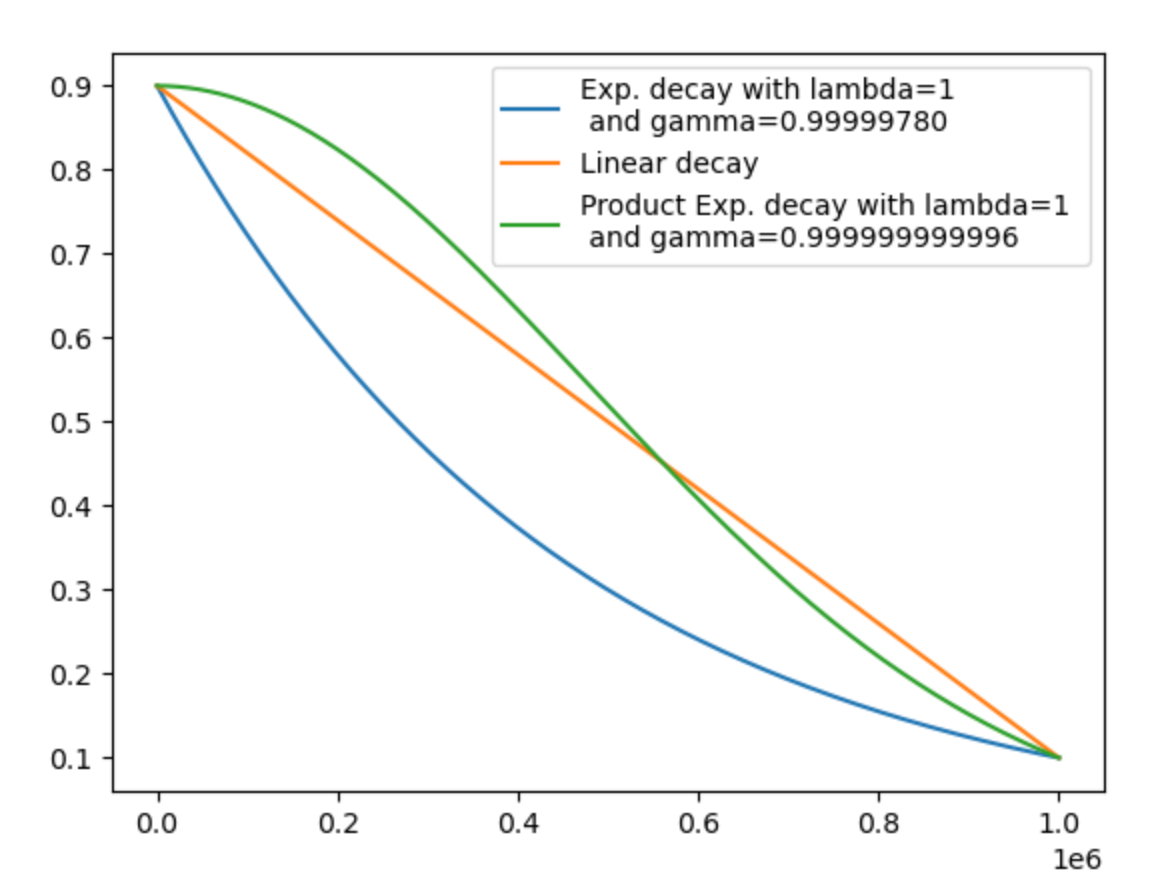
\includegraphics[width=0.7\linewidth]{figures/shape_exploration_functions}
	\caption{Shape of the proposed exploration functions for the DQN agent}
	\label{fig:shape_exp_funs}
\end{figure}

\subsection{Extracting explainability features}
In this section we are going to explain how, once we trained our models, we extracted several feature maps to understand what the model is taking into account to perform an action. We must note that for section \ref{sec:extracting_attn_maps}, we could not implement a way to extract raw attention maps for the SWIN transformer, nor we found any reference in the literature that would help us with this purpose, so we only extracted the attention maps for the ViT model. For section \ref{sec:grad_cam_act_maps}, the developed method takes into account both ViT and SWIN transformer.

\subsubsection{Extracting attention maps}
\label{sec:extracting_attn_maps}
As explained in section \ref{sec:vis-transformers}, the ViT introduces an additional token along the patches, called the class token, which holds the information that class takes into account via self-attention to produce the output. Figure \ref{fig:classtokenattention} illustrates this, since we can see that, for a 4 by 4 patched image, the disposition of the attention matrix for one attention head would give us for the class token row, all the patches with the weighted attention. The code developed for this section is available in the script \href{https://github.com/Javimh18/DL_TFM/blob/main/src/visualize_attention_vit.py}{visualize\_attention\_vit.py}.

\begin{figure}[!h]
	\centering
	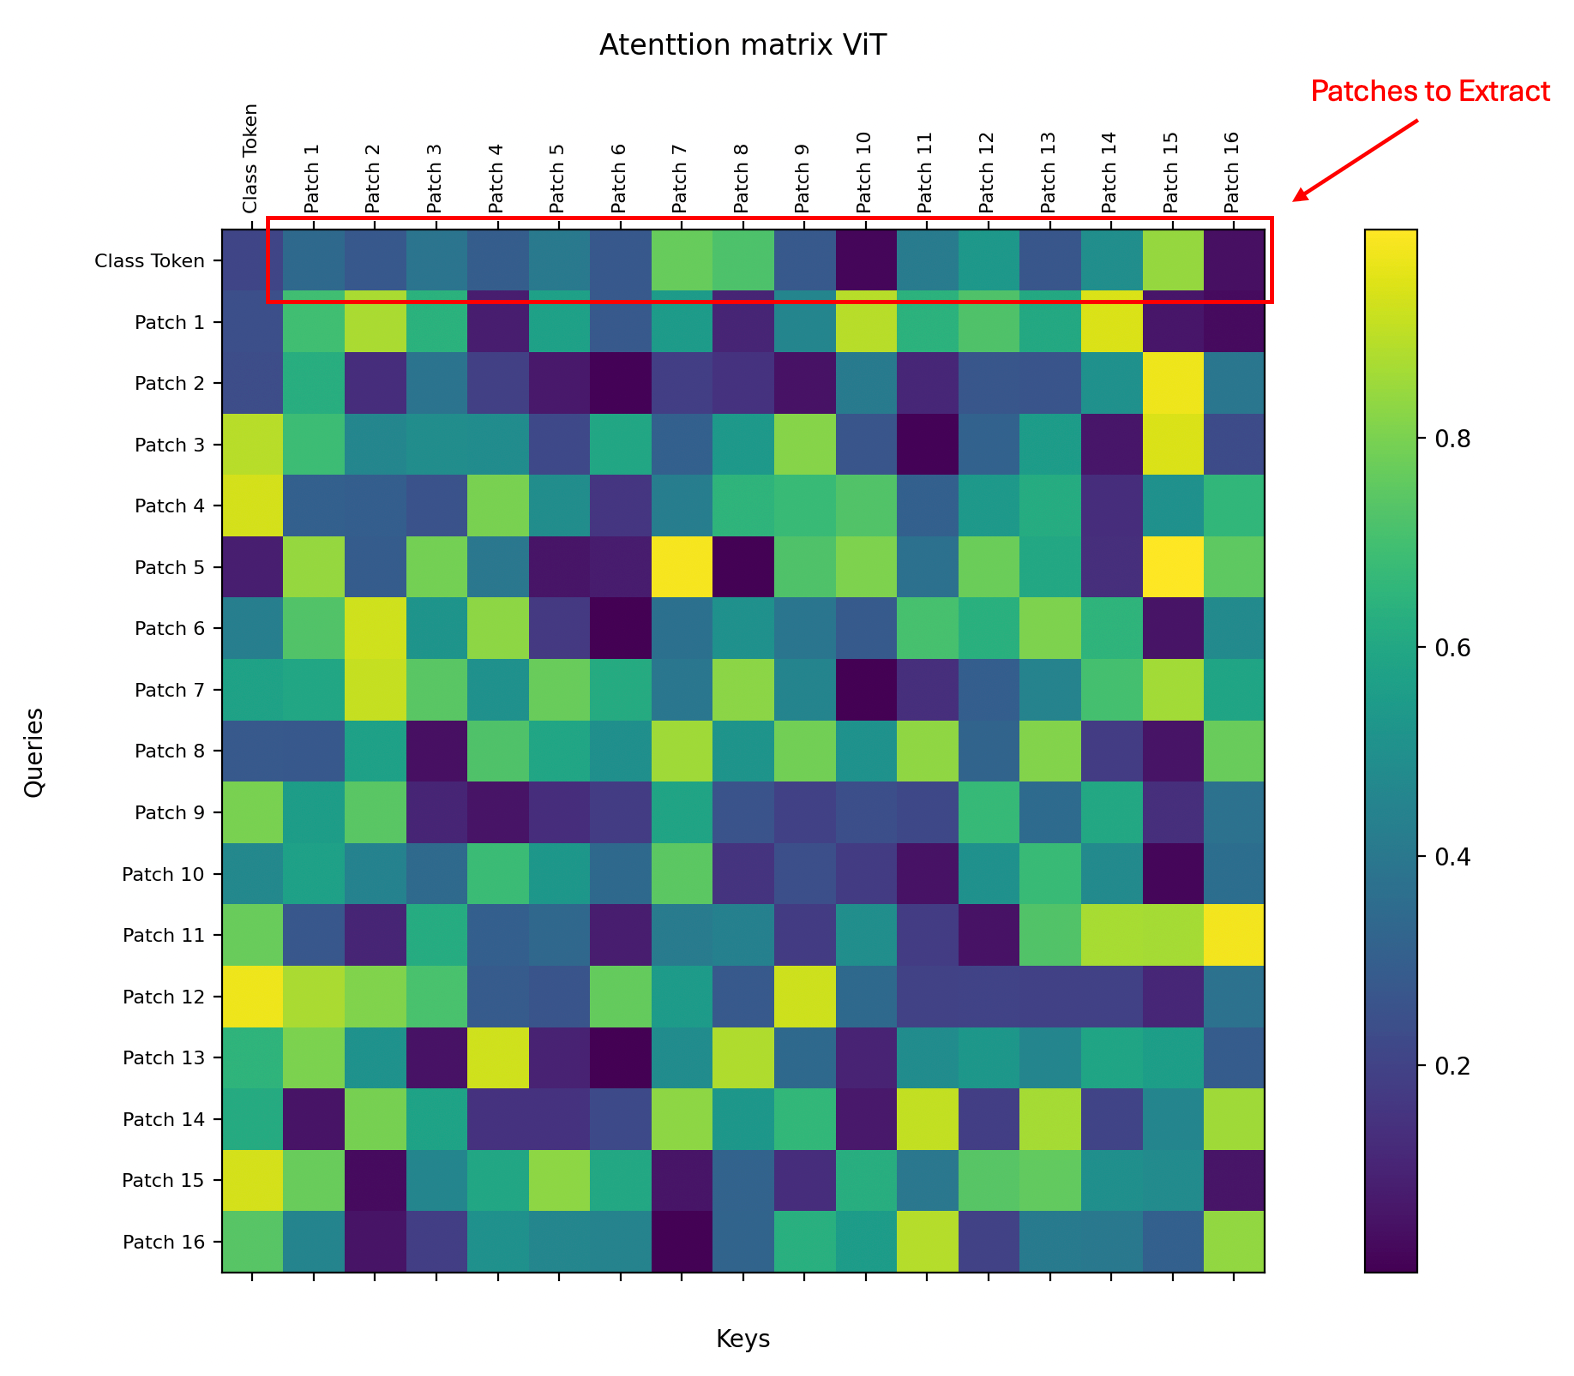
\includegraphics[width=0.7\linewidth]{figures/class_token_attention}
	\caption{Example of an attention matrix for one attention head with 4 $\times$ 4 patches. The section under the red rectangle refers to the patches that the class token ponders in order to perform the output. This patches will be our extraction for the attention maps.}
	\label{fig:classtokenattention}
\end{figure}

In order to extract the attention maps, the implementation from \cite{caron2021emerging} has the functionality of returning the attention maps in the forward pass of the ViT blocks (see listing \ref{code:attn_block}). The only thing we ought to do, is index the attention matrix correctly to extract the elements of interest. In listing \ref{code:single_frame_attn}, we can see a example of this. First, we obtain the attention weights for each patch by indexing the attention matrix like \inlinecode{attn[0, :, 0, 1:]} in line 3, obtaining a matrix with dimensions $\mathbb{R}^{nh \times (P-1)}$, where nh refers to the number of heads from the attention mechanism, and P refers to the tokens that go into the attention mechanism. Since we are not interested in the attention weight that the class token has with respect to itself, we exclude it out. To compute the averaged importance of each patch, we perform the mean across the nh dimension, and reshape the $P$ dimension to the original spatial dimensions $P_w$ and $P_h$ for the width and the height respectively (line 4). Then, by calling the method \inlinecode{interpolate_attn_map} we perform a interpolation to return the attention map to the original size of the input (lines 5 to 8).

\begin{lstlisting}[caption={Attention map extractor for a single frame}, label={code:single_frame_attn}]
	vit = agent.net.online
	attn = vit.get_last_selfattention(state.float())
	cls_attn = attn[0, :, 0, 1:]
	cls_attn = cls_attn.reshape(-1, dimension, dimension).mean(dim=0, keepdim=True).unsqueeze(0)
	# 3. Interpolate the attention maps to original frame size
	cls_attn_int = interpolate_attn_map(attention_map=cls_attn, 
	scale_factor=patch_size,
	final_shape=original_shape)
\end{lstlisting}

Once we have done this, we can plot the attention map along with the original frame to observe where does the model pay attention to, given a frame. In Figure \ref{fig:attnvisualizationframe} we provide an example for this. Additionally, in the right side of the figure, we provide the returned Q-values from the network, since they are of vital importance for understanding the network's decisions. The interpretations that we extract from this will be discussed in section \ref{cha:evaluation}.

\begin{figure} [!h]
	\centering
	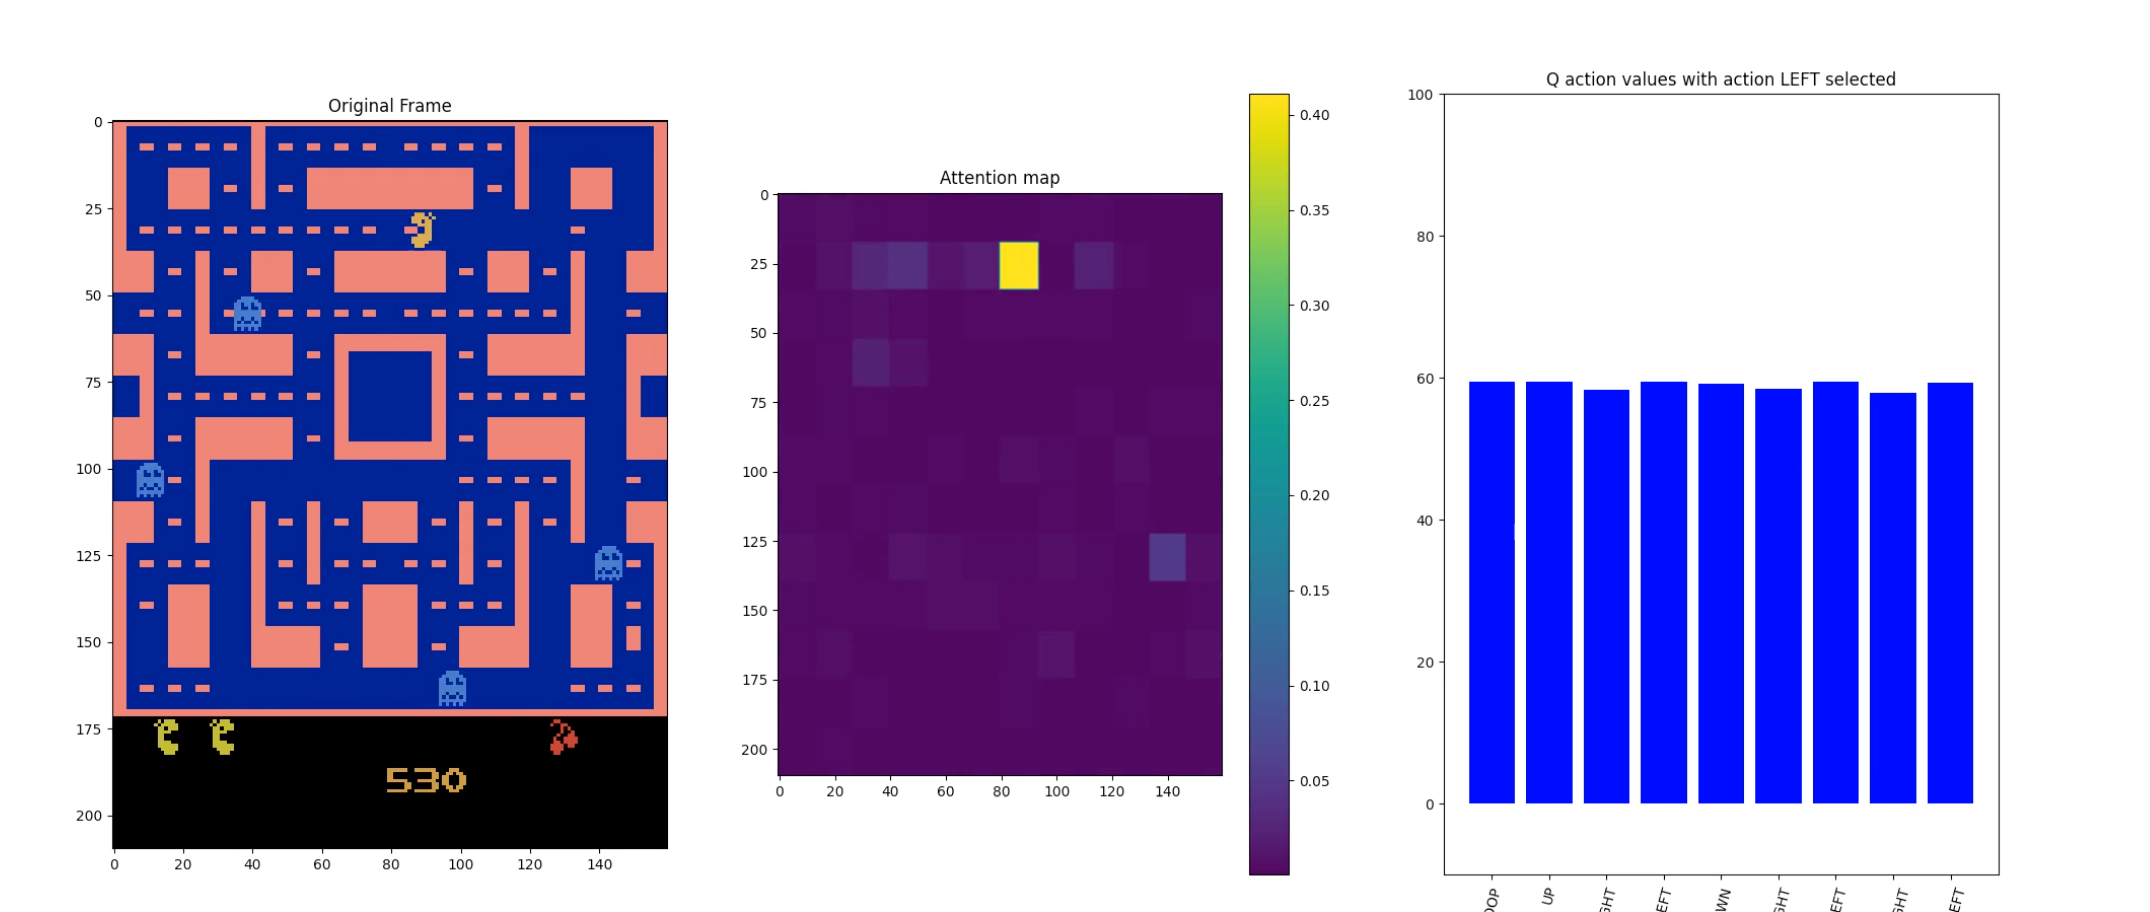
\includegraphics[width=\linewidth]{figures/attn_visualization_frame}
	\caption{Left side, the original frame from the game, in the center, the attention maps for the class token, at the right-side, the Q-values for the observation from the state.}
	\label{fig:attnvisualizationframe}
\end{figure}



\subsubsection{Extracting Grad-CAM's activation maps}
\label{sec:grad_cam_act_maps}
We developed something similar to section \ref{sec:extracting_attn_maps} but using the grad-CAM technique explained in \ref{sec:cam}. To do so, we used the \inlinecode{pytorch-cam} library \cite{jacobgilpytorchcam} that integrates a well varied amount of CAM methods to select. Part of the developed code is displayed in listing \ref{code:grad_cam_rl}, and the complete code can be found in the \href{https://github.com/Javimh18/DL_TFM/blob/main/src/visualize_activations.py}{visualize\_activations.py} script.

\begin{lstlisting}[caption={Activation maps using Grad-CAM}, label={code:grad_cam_rl}]
	action, q_v = agent.perform_action(state, t=-1, exploit=True)
	actions.append(action)
	q_values.append(q_v.squeeze().detach().cpu().numpy())
	# 2. get the activation maps
	state = first_if_tuple(state).__array__()
	state = torch.tensor(np.array([state]), device=device)
	action_target = ClassifierOutputTarget(action)
	gray_scale_cam = cam(input_tensor=state, targets=[action_target])
	gray_scale_cam = torch.tensor(gray_scale_cam[0, :]).unsqueeze(0).unsqueeze(0) # appropiate dims for interpolation
	activ_map = interpolate_activations(gray_scale_cam,
	final_shape=original_shape)
\end{lstlisting}

To adapt Grad-CAM from the classification supervised learning set-up to the reinforcement learning set-up, we treated each of the actions the agent selected as the predicted "class". By doing so, we expected to obtain the biggest activations from the input that the agent considers to perform the output. The \inlinecode{ClassifierOutputTarget} method takes the target class (our action in this case), and passes it to the cam method, that returns the activations. Then we perform an interpolation to return the resolution to the original frame size, obtaining a map depicted in Figure \ref{fig:activationmapsvisualization}. We must say that this method works for both ViT and SWIN backbones, along with other non-attention based models, such as CNNs. 

\begin{figure}[!h]
	\centering
	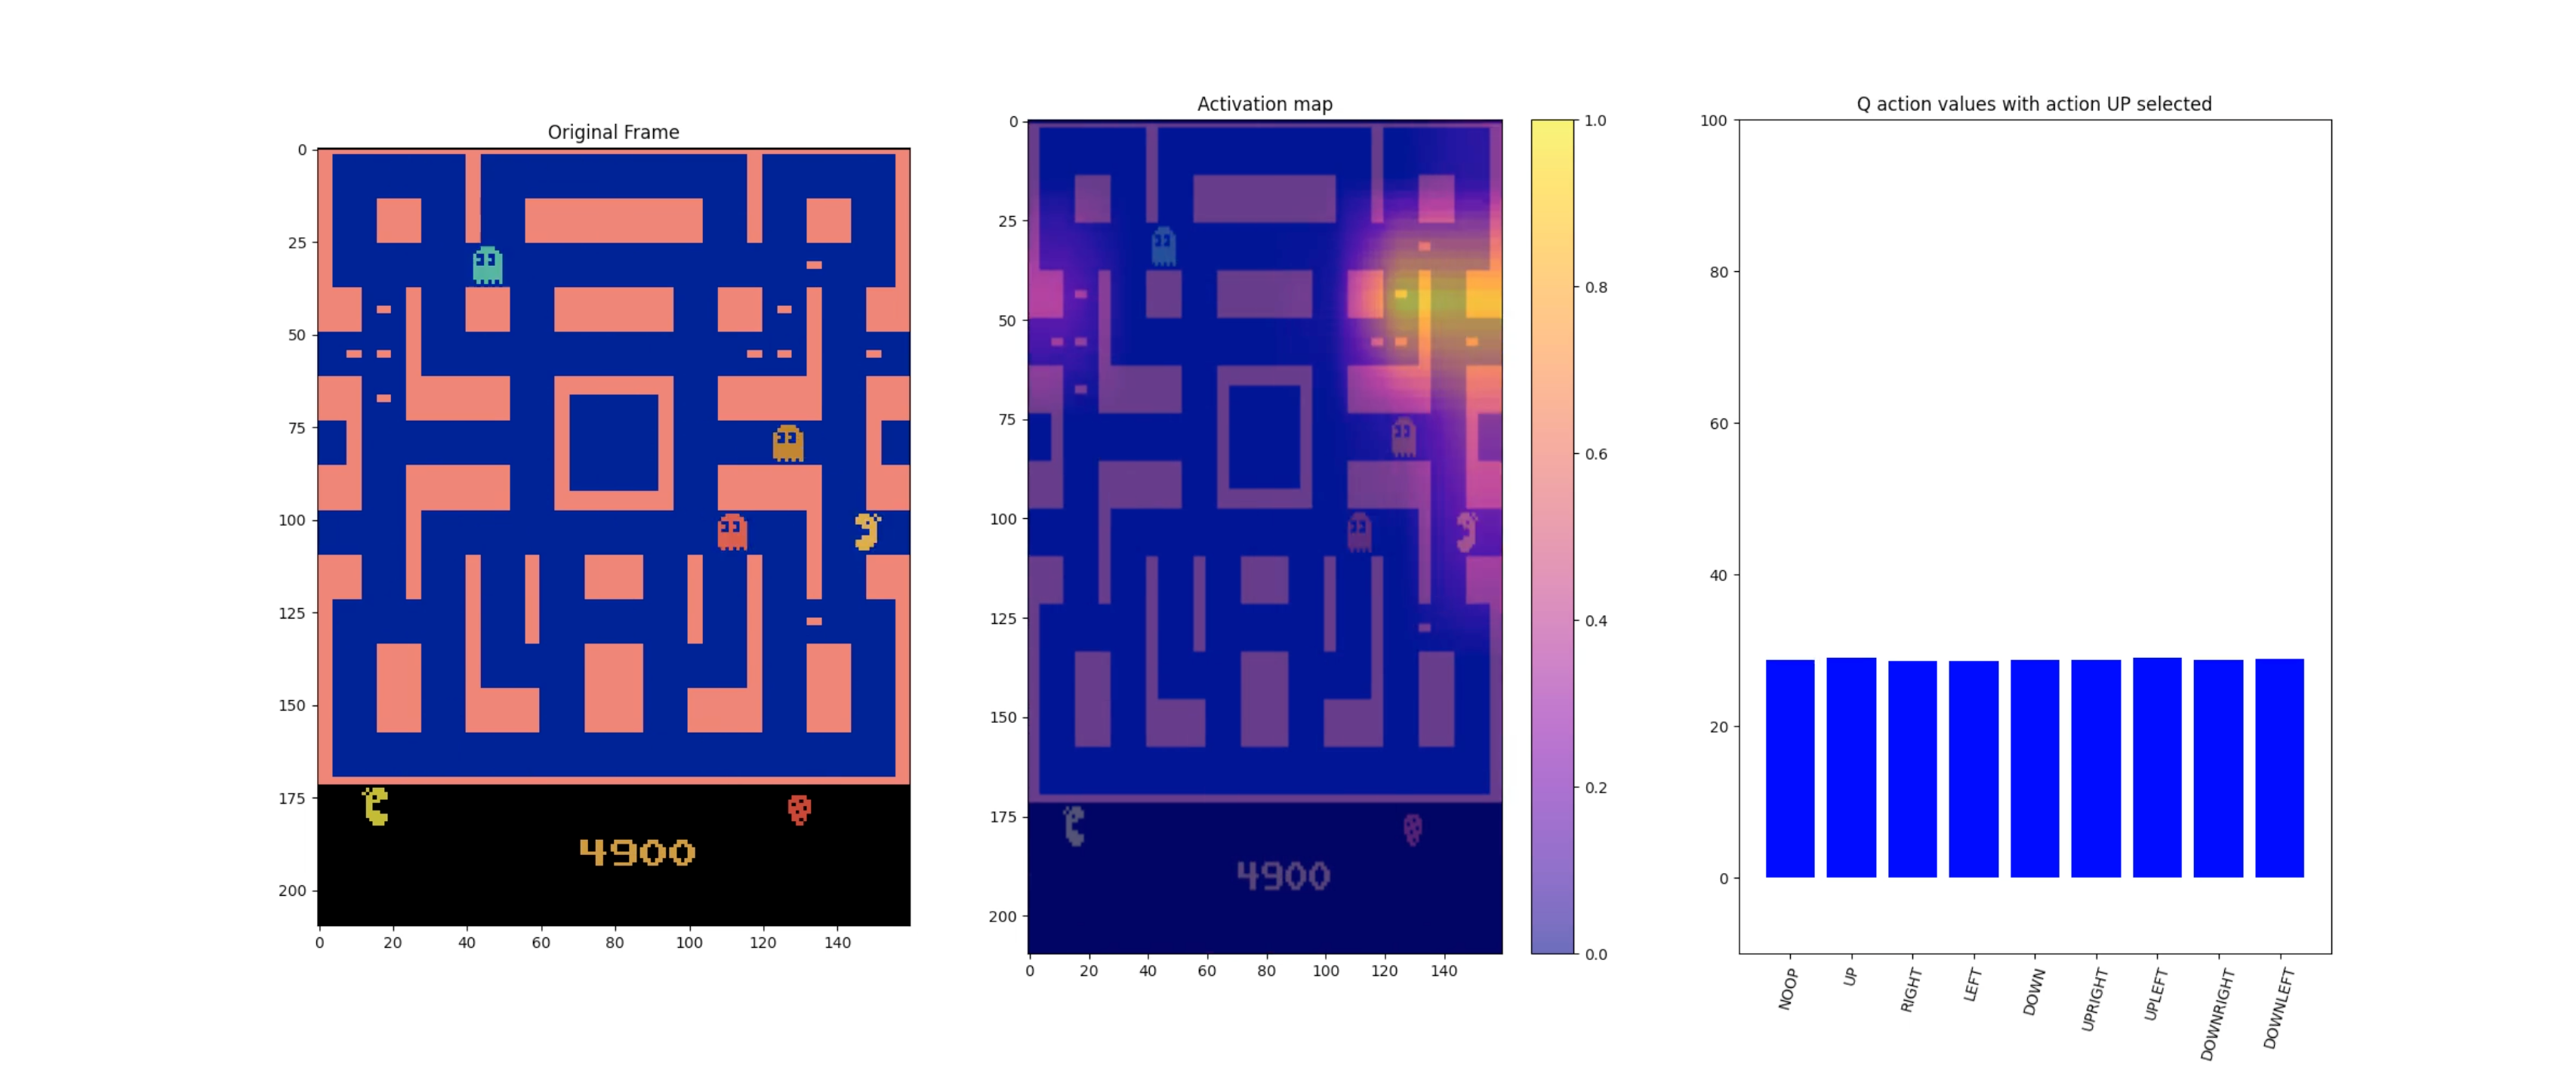
\includegraphics[width=\linewidth]{figures/activation_maps_visualization}
	\caption{Left-side, the current frame of the game. In the center, the activation maps from the ViT using grad-CAM. At the right-side, the Q-values provided by the neural network.}
	\label{fig:activationmapsvisualization}
\end{figure}


\subsection{Additional implementations}

\subsubsection{Configuration files}
As explained in sections \ref{sec:vit_transformer_imp} and \ref{sec:swin_transformer_rl}, the implementation of these models is highly parametrizable, since we can state lots of parameters that are involved in the topology of the models. Changing these parameters manually in each file is a burden, since we have to check that the changes are done correctly in the several files involved in running the training process. To tackle this issue, we proposed two files: one for the DQN agent hyper-parameters, and another for the models hyper-parameters called \href{https://github.com/Javimh18/DL_TFM/blob/main/config/agents_config.yaml}{agents\_config.yaml} and \href{https://github.com/Javimh18/DL_TFM/blob/main/config/agent_nns.yaml}{agent\_nns.yaml}.
For loading this files, we used the \inlinecode{pyyaml} library, that eases a lot the loading a manipulation of yaml files, and used them properly to initialize the corresponding hyper-parameters, such as number of steps for training, the learning rate for the back-propagation and the Q-estimates or the number of layers that our model will have. Thanks to this implementation, we were able to seamlessly change the configuration of the agents, allowing for room to explore different hyper-parameters configurations.

\subsubsection{Checkpoints}
As the training process progresses, the weights of our function approximators will change. There are some cases where the excess of training produces a degradation on the model's performance, ending the training with a sub-optimal model. To change this, we implemented a checkpoint saver in our pipeline, that saves periodically the model's state dictionary, that contains the weights of the model. By doing a snap-shot of the model weights, we have several versions, which will be of use when we run our evaluations of the agents in the environment. Additionally, the checkpoints are of great use if we want to resume a training process. We have also developed adaptations to our code that perform these kinds of operations, and have been of great use when unexpected events (such as lack of computational resources) stopped our training process.

\subsection{Overview}
\label{sec:overview_implementation}

With almost all the components involved in the training pipeline for our agents, in Figure \ref{fig:implementationoverview} we present the diagram of all the modules developed along with their relationships. 

\begin{figure}[!h]
	\centering
	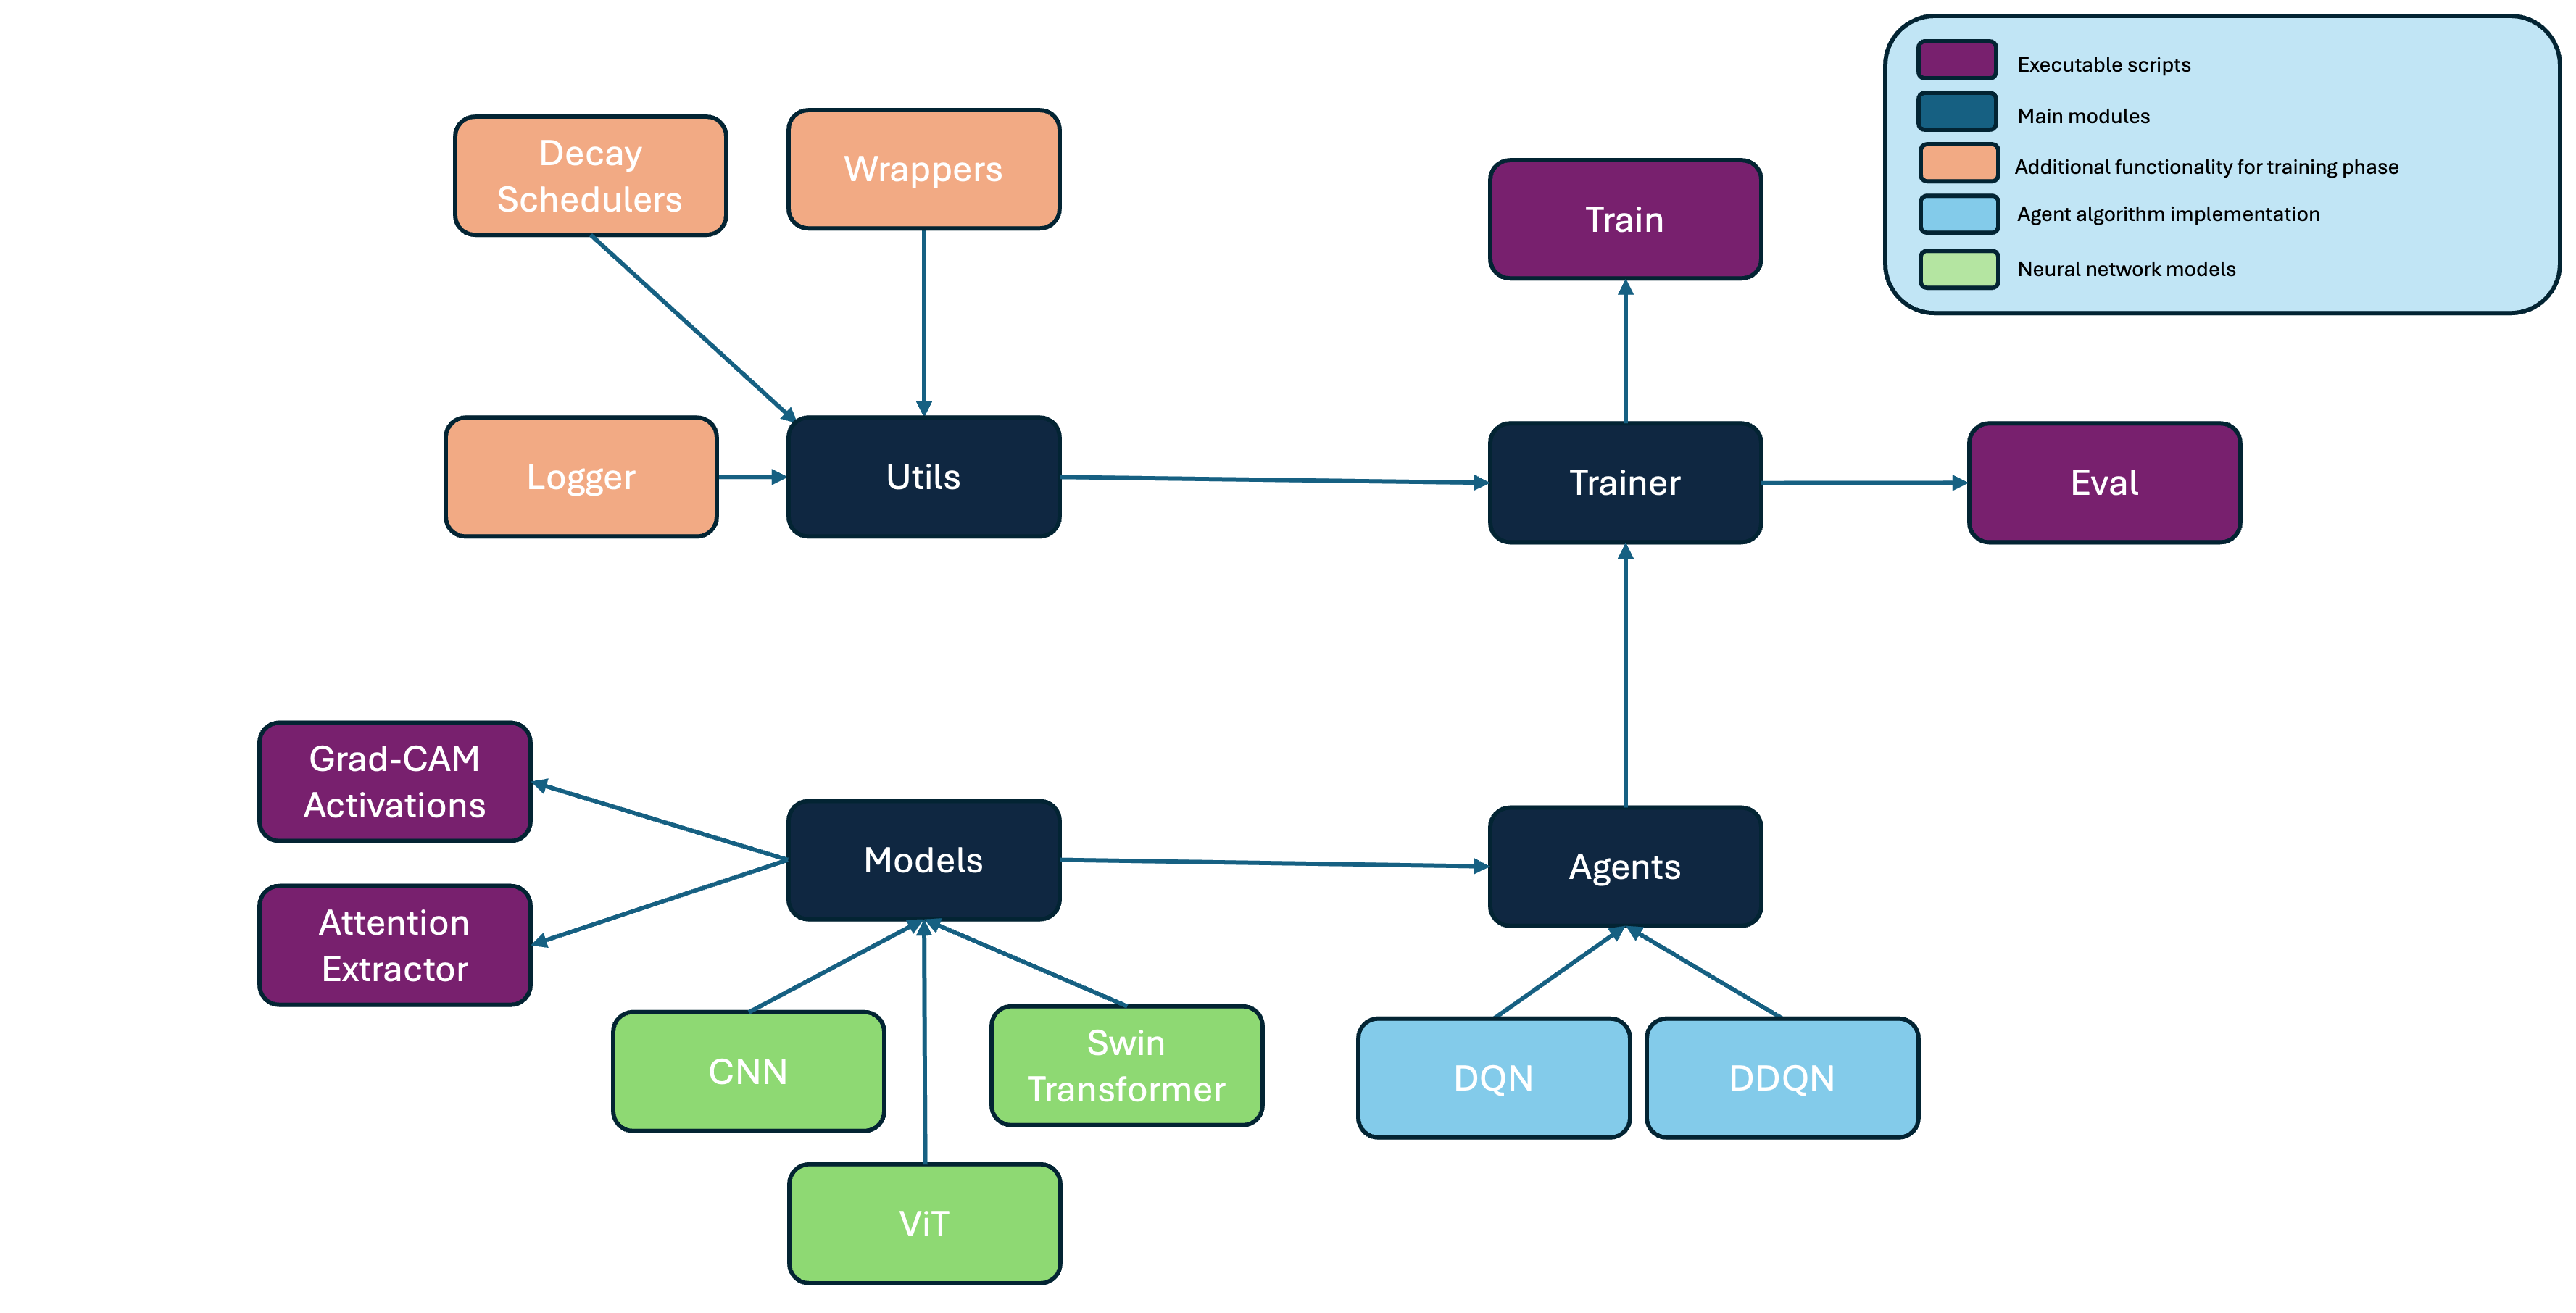
\includegraphics[width=\linewidth]{figures/implementationoverview}
	\caption{Implementation overview of all the modules involved in this work}
	\label{fig:implementationoverview}
\end{figure}





